% !TEX root = ../OT4ML.tex

\chapter{Beyond Comparing Measures}
\label{sec-beyond-comparing-measures}

This chapter leaves the setting of scalar measures on a common ambient space. Vector- and matrix-valued OT transports mass with internal degrees of freedom, Gromov--Wasserstein compares metric-measure spaces without a prescribed correspondence, and quantum OT replaces scalar couplings by positive operators. In each case, the transport plan must also encode structure carried by the support, the fibers or the non-commutative state space.
\index{positive!operator}% strictindex
\index{plan!transport}% strictindex
\index{correspondence}% strictindex
\index{quantum!OT}% strictindex
\index{metric-measure space}% strictindex
\index{Gromov-Wasserstein@Gromov--Wasserstein}% strictindex
\index{Gromov-Wasserstein@Gromov--Wasserstein!distance}% strictindex

\section{Vector and Matrix-Valued Measures}
\index{vector-valued measure}% strictindex
\index{matrix-valued measure}% strictindex
\label{sec-vector-matrix-valued-measures}

Scalar OT transports a nonnegative density. In imaging, color processing, spectral analysis, diffusion tensor imaging and quantum-inspired models, the object attached to a point can instead have several nonnegative components or a positive semidefinite matrix. The first step beyond scalar OT is the positive vector-valued case: the fiber remains linear and commutative, but the transport cost may couple its channels.
\index{positive!semidefinite matrix}% strictindex

\paragraph{Positive vector-valued measures.}
\index{positive!vector-valued measure}% strictindex

The simplest way to keep internal structure in transport is to attach several nonnegative masses to each spatial point and to decide whether these channels move independently or interact through the cost.
\begin{defn}[Positive vector-valued measure]\label{def-positive-vector-valued-measure}
\index{vector-valued measure}% strictindex
	A positive $\RR_+^m$-valued measure on $\X$ is a tuple
	\[
		\al=(\al^1,\ldots,\al^m)\in\Mm_+(\X;\RR_+^m),
	\]
	where each component $\al^k$ is a nonnegative finite measure.
\end{defn}
This models multi-channel densities such as color histograms, spectral bins or several species transported on the same domain. In a conservative model the mass of each channel is preserved, so one assumes $\al_0^k(\X)=\al_1^k(\X)$ for every $k$. The natural vector-valued extension of OT therefore starts from the positive cone $\RR_+^m$.
\index{finite measure}% strictindex
\index{histogram}% strictindex
\index{positive!cone}% strictindex

For the dynamic formulas below, assume that $\X$ is either $\RR^d$, the flat torus, or a bounded convex domain in $\RR^d$ equipped with no-flux boundary conditions. First suppose that the endpoints and the curve have densities. The direct analogue of Benamou--Brenier fixes a vector density $u_t(x)\in\RR_+^m$ and a spatial flux
\index{flux}% strictindex
\index{Benamou-Brenier@Benamou--Brenier}% strictindex
$V_t(x)=(V_{t,1},\ldots,V_{t,d})\in(\RR^m)^d$, where $V_{t,\ell}^k$ is the momentum of channel $k$ in spatial direction $\ell$. The conservative vector transport cost associated with an action density $\Phi$ is
\index{momentum}% strictindex
\begin{defn}[Vector-valued dynamic transport]\label{def-vector-valued-dynamic-transport}
For a nonnegative extended-valued action density $\Phi:\RR_+^m\times(\RR^m)^d\to[0,+\infty]$, define
\begin{equation}\label{eq-vector-valued-bb}
	\mathcal W_{\Phi}^2(\al_0,\al_1)
	\eqdef
	\inf_{u,V}
	\int_0^1\!\int_\X
	\Phi(u_t(x),V_t(x))\,\d x\,\d t
\end{equation}
subject to the endpoint constraints $u_0\d x=\al_0$, $u_1\d x=\al_1$ and the componentwise continuity equation
\index{continuity equation}% strictindex
\begin{equation}\label{eq-vector-valued-continuity}
	\partial_t u_t+\nabla_x\cdot V_t=0,
	\qquad
	(\nabla_x\cdot V_t)^k=\sum_{\ell=1}^d \partial_{x_\ell} V_{t,\ell}^k .
\end{equation}
\end{defn}
Thus each component satisfies its own continuity equation, but the cost may still couple the components. Singular curves are handled as in scalar dynamic OT by replacing densities and fluxes by measures and using the lower semicontinuous perspective recession convention.
\index{perspective recession}% strictindex
\index{recession convention}% strictindex
\index{flux}% strictindex
\index{lower semicontinuity}% strictindex
\index{continuity equation}% strictindex

The following elementary family separates independent channel motion from genuinely coupled vector transport.

\begin{example}[Diagonal and coupled positive mobilities]
Choose a mobility matrix $\mathsf M(u)\in\mathbb S_+^m$, where $\mathbb S_+^m$ denotes the cone of real symmetric positive semidefinite matrices, and set
\index{positive!semidefinite matrix}% strictindex
\[
	\Phi_{\mathsf M}(u,V)
	=
	\sum_{\ell=1}^d V_{\ell}^{\top}\mathsf M(u)^\dagger V_{\ell},
\]
with the usual convention that the value is finite only when each $V_\ell$ belongs to the range of $\mathsf M(u)$. If $u\mapsto\mathsf M(u)$ is linear and takes values in $\mathbb S_+^m$, then this action is jointly convex and positively one-homogeneous in $(u,V)$. Indeed, the matrix fractional map $(M,z)\mapsto z^\top M^\dagger z$ is jointly convex on its effective domain, and linearity gives $\mathsf M(su)=s\mathsf M(u)$ for $s>0$. For $m=1$ and $\mathsf M(u)=u$, one recovers exactly the scalar Benamou--Brenier action. For
\index{Benamou-Brenier@Benamou--Brenier}% strictindex
\[
	\mathsf M_{\mathrm{diag}}(u)=\diag(u_1,\ldots,u_m),
\]
the channels move independently. Non-diagonal mobilities are the simplest way to couple the coordinates while keeping the same componentwise conservation law. For instance, with $q=m^{-1/2}(1,\ldots,1)$ and $\kappa\geq0$,
\[
	\mathsf M_\kappa(u)=\diag(u)+\kappa\Big(\sum_{k=1}^m u_k\Big) q q^\top
\]
increases the mobility in the common channel direction $q$ while leaving transverse directions controlled by the diagonal part. The local cost of moving one component can therefore depend on the densities and momenta of the other components, even though each component mass remains conserved.
\index{momentum}% strictindex
\end{example}

\begin{prop}[Diagonal positive vector Benamou--Brenier]\label{prop-diagonal-positive-vector-bb}
\index{Benamou-Brenier@Benamou--Brenier}% strictindex
Assume that $\al_0^k,\al_1^k\in\Mm_+(\X)$ have finite second moments and the same mass $m_k$ for every $k$. For the diagonal mobility $\mathsf M_{\mathrm{diag}}$, the value of~\eqref{eq-vector-valued-bb} is
\[
	\mathcal W_{\mathrm{diag}}^2(\al_0,\al_1)
	=
	\sum_{k:m_k>0} m_k\,\Wass_2^2\!\left(\frac{\al_0^k}{m_k},\frac{\al_1^k}{m_k}\right),
\]
with the convention that zero-mass channels contribute zero.
\end{prop}
\begin{proof}
For $\mathsf M_{\mathrm{diag}}(u)=\diag(u_1,\ldots,u_m)$, the action separates as
\[
	\sum_{\ell=1}^d V_\ell^\top \mathsf M_{\mathrm{diag}}(u)^\dagger V_\ell
	=
	\sum_{k=1}^m \frac{|V^k|^2}{u^k},
\]
where $V^k=(V_1^k,\ldots,V_d^k)$ is the spatial momentum of channel $k$, and the scalar perspective convention is used. The constraint~\eqref{eq-vector-valued-continuity} also separates into $\partial_t u^k+\nabla\cdot V^k=0$. The minimization therefore splits into $m$ independent scalar Benamou--Brenier problems. If $m_k=0$, nonnegativity and conservation force the whole channel to vanish. If $m_k>0$, normalizing $\rho_t^k=u_t^k/m_k$ and $p_t^k=V_t^k/m_k$ factors the channel action as $m_k\int |p_t^k|^2/\rho_t^k$, hence the scalar value is $m_k\Wass_2^2(\al_0^k/m_k,\al_1^k/m_k)$. Summing over the channels proves the claim.
\index{momentum}% strictindex
\index{Benamou-Brenier@Benamou--Brenier}% strictindex
\end{proof}

The conservative positive-cone model above is the basic extension of Benamou--Brenier. Adding a source term $\partial_t u+\nabla\cdot V=S$ and a convex perspective penalty in $S$ gives unbalanced or reaction--transport variants. Such generalized transport models with dissipation and density modulation were developed by Maas, Rumpf, Sch{\"o}nlieb and Simon~\cite{maas2015generalized,maas2016generalized}; related nonlinear mobility distances and gradient structures appear in~\cite{dolbeault2009new,MielkeCVPDE}. Figure~\ref{fig:vector-valued-measure-geodesics} contrasts the exact diagonal case $\kappa=0$, where each positive channel is transported by its quantile map, with a large-$\kappa$ illustrative common-mode interpolation in which the channels move more coherently. The endpoints are two-mode mixtures: at each spatial mode the two channels have Gaussian profiles with the same center but different amplitudes.
\index{gradient!structure}% strictindex
\index{vector-valued measure}% strictindex
\index{positive!cone}% strictindex
\index{quantile!map}% strictindex

\begin{figure}[H]
\centering
\begin{tabular}{@{}cc@{}}
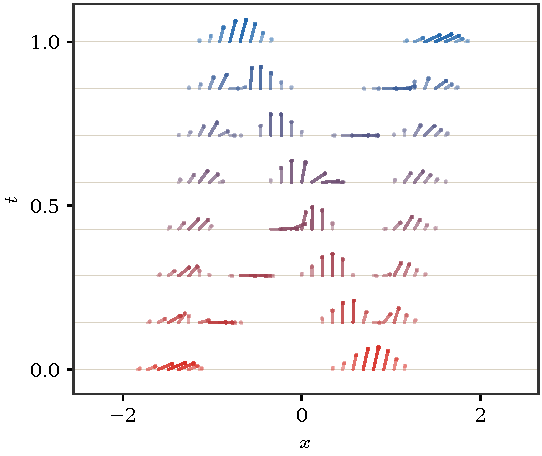
\includegraphics[width=.45\linewidth]{figures/vector-valued-measure-geodesics/kappa-zero-arrows.pdf} &
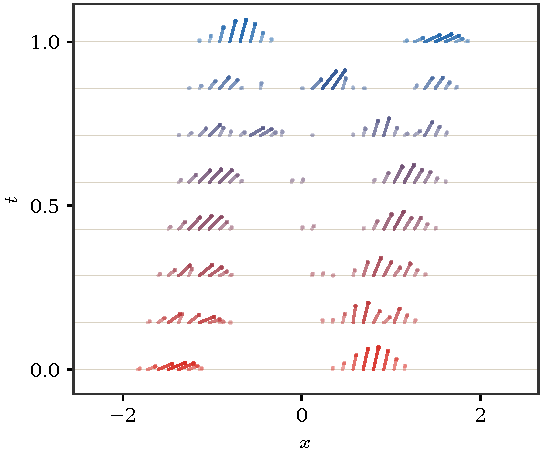
\includegraphics[width=.45\linewidth]{figures/vector-valued-measure-geodesics/kappa-large-arrows.pdf}
\\[-.1em]
\small independent channels $(\kappa=0)$ &
\small strongly coupled channels $(\kappa\gg1)$
\end{tabular}
\caption{\emph{One-dimensional positive $\RR_+^2$-valued transport displayed by arrow glyphs at eight time levels.} Each endpoint is a mixture of two localized Gaussian modes, and, inside each mode, both channel profiles have the same center. Each arrow is proportional to the local fiber value $(u_t^1(x),u_t^2(x))$, and time runs vertically from the red source to the blue target. Left: for $\kappa=0$, the diagonal mobility of Proposition~\ref{prop-diagonal-positive-vector-bb} gives two independent scalar quantile geodesics. Right: a large-$\kappa$ common-mode interpolation bends the display toward the direction $q=2^{-1/2}(1,1)$, illustrating the qualitative effect of a mobility that favors coherent channel motion while keeping the same componentwise continuity equation.}
\index{continuity equation}% strictindex
\label{fig:vector-valued-measure-geodesics}
\end{figure}

\paragraph{Positive matrix-valued measures.}
\index{matrix-valued measure}% strictindex
\index{positive!matrix-valued measure}% strictindex
The next simplest fiber is the positive matrix cone. This is the simplest tensor-valued model beyond vectors: the diagonal entries behave like positive channels, while the eigenvectors encode local orientations.

\begin{defn}[Positive matrix-valued measure]\label{def-positive-matrix-valued-measure}
\index{matrix!cone}% strictindex
	Write $\mathbb S^m$ for real symmetric matrices and $\mathbb S_+^m$ for the positive semidefinite cone. A positive $\mathbb S_+^m$-valued measure is a countably additive map from Borel sets of $\X$ to $\mathbb S_+^m$; we denote the cone of such measures by
	\[
		\mathcal A\in\Mm_+(\X;\mathbb S_+^m).
	\]
\end{defn}
Equivalently, $\mathcal A$ is a symmetric matrix of finite signed measures such that $\mathcal A(E)\succeq0$ for every Borel set $E$. If $\mathcal A$ has density $A(x)\succeq0$, then $\tr A(x)$ is the scalar amount of mass at $x$, while, wherever $\tr A(x)>0$, the normalized matrix $A(x)/\tr A(x)$ records an internal covariance or orientation. This is the matrix analogue of the positive vector case: diagonal matrices encode nonnegative vector components, and non-diagonal matrices add a local eigenbasis.

The conservative Benamou--Brenier model fixes a matrix density $A_t(x)\in\mathbb S_+^m$ and symmetric matrix fluxes $P_t(x)=(P_{t,1},\ldots,P_{t,d})\in(\mathbb S^m)^d$. With no flux through the boundary of $\X$, the full matrix mass $\int_\X A_t(x)\d x$ is conserved, so the endpoints must have the same total matrix. The resulting matrix-perspective problem is the following.
\index{flux}% strictindex
\index{Benamou-Brenier@Benamou--Brenier}% strictindex
\begin{defn}[Matrix-valued dynamic transport]\label{def-matrix-valued-dynamic-transport}
\begin{equation}\label{eq-matrix-valued-bb}
\begin{aligned}
\mathcal W_{\mathrm{mat}}^2(\mathcal A_0,\mathcal A_1)
\eqdef
\inf_{A,P}\int_0^1\!\int_\X
\sum_{\ell=1}^d \tr\big(P_{t,\ell}^{\top} A_t^\dagger P_{t,\ell}\big)\d x\d t
\end{aligned}
\end{equation}
subject to $A_0\d x=\mathcal A_0$, $A_1\d x=\mathcal A_1$ and to the matrix-valued continuity equation
\index{matrix-valued measure}% strictindex
\index{continuity equation}% strictindex
\begin{equation}\label{eq-matrix-valued-continuity}
\partial_t A_t+\nabla_x\cdot P_t=0,
\qquad
\nabla_x\cdot P_t=\sum_{\ell=1}^d \partial_{x_\ell}P_{t,\ell}.
\end{equation}
Here $A_t^\dagger$ is the Moore--Penrose inverse, and the integrand is $+\infty$ unless
$\operatorname{Ran}(P_{t,\ell})\subseteq\operatorname{Ran}(A_t)$ for every $\ell$.
\end{defn}
This is the usual lower-semicontinuous perspective convention. The matrix fractional map $(A,P)\mapsto\tr(P^{\top}A^\dagger P)$ is jointly convex on this effective domain and positively one-homogeneous in $(A,P)$. This gives the simplest non-trivial matrix-valued transport model: spatial motion is conservative, but the fiber carries orientation through the eigenvectors of $A_t(x)$.

\begin{prop}[Diagonal matrix subproblem]\label{prop-matrix-diagonal-reduction}
\index{matrix!subproblem}% strictindex
Assume that the endpoints are diagonal in a fixed orthonormal basis,
\[
	\mathcal A_i=\diag(\al_i^1,\ldots,\al_i^m),
	\qquad i=0,1,
\]
and that $\al_0^k(\X)=\al_1^k(\X)=m_k$ for every $k$. If one restricts the admissible curves in~\eqref{eq-matrix-valued-bb} to remain diagonal in that basis,
\[
	A_t=\diag(u_t^1,\ldots,u_t^m),
	\qquad
	P_{t,\ell}=\diag(V_{t,\ell}^1,\ldots,V_{t,\ell}^m),
\]
then the value of this restricted matrix problem is
\[
	\sum_{k:m_k>0} m_k\,\Wass_2^2\!\left(\frac{\al_0^k}{m_k},\frac{\al_1^k}{m_k}\right),
\]
with zero contribution from zero-mass channels. Thus the commuting matrix submodel is exactly the diagonal positive vector-valued Benamou--Brenier model of Proposition~\ref{prop-diagonal-positive-vector-bb}.
\index{Benamou-Brenier@Benamou--Brenier}% strictindex
\end{prop}
\begin{proof}
The continuity equation~\eqref{eq-matrix-valued-continuity} is diagonal entry by diagonal entry and gives $\partial_t u^k+\nabla\cdot V^k=0$. Moreover,
\index{continuity equation}% strictindex
\[
	\sum_{\ell=1}^d \tr\big(P_{t,\ell}^{\top}A_t^\dagger P_{t,\ell}\big)
	=
	\sum_{k=1}^m \frac{|V_t^k|^2}{u_t^k}
\]
with the same scalar perspective convention as before. The admissible set and the action are therefore exactly those of the diagonal vector model.
\end{proof}

The restriction to a fixed diagonal basis gives eigenvalue transport; it should be read as a commuting submodel, not as a claim that non-diagonal excursions can never change the unrestricted value. The genuinely matrix-valued case starts when the eigenspaces vary with $x$ or along the interpolation, so that the transported object carries both mass and orientation. Static matrix-valued Monge--Kantorovich problems and dual test-function metrics were developed in~\cite{Ning2014metrics,JiangSpectral,ning2015matrix}; dynamic versions and related non-commutative geometries appear in~\cite{Chen2016,ChenGangbo17,Carlen2014,2016-peyre-qot}. Figure~\ref{fig:matrix-valued-measure-geodesic} shows the analogous independent/coupled contrast for positive $2\times2$ matrix fibers, using two localized matrix modes whose eigenvalue profiles share a common center at each mode.
\index{Kantorovich!problem}% strictindex
\index{matrix-valued measure}% strictindex

\begin{figure}[H]
\centering
\begin{tabular}{@{}cc@{}}
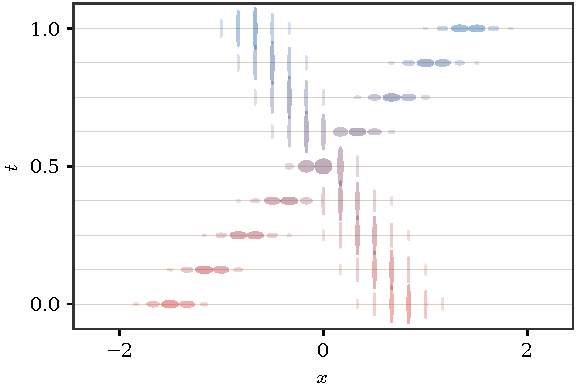
\includegraphics[width=.46\linewidth]{figures/matrix-valued-measure-geodesic/independent-ellipses.pdf} &
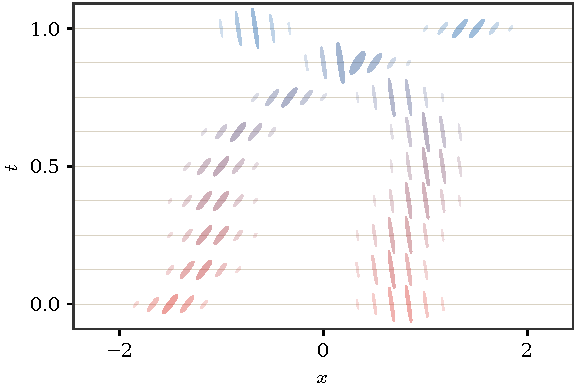
\includegraphics[width=.46\linewidth]{figures/matrix-valued-measure-geodesic/coupled-ellipses.pdf}
\\[-.1em]
\small commuting tensor channels &
\small strongly coupled tensor fibers
\end{tabular}
\caption{\emph{Positive $2\times2$ matrix-valued transport on a one-dimensional base.} Each endpoint is a mixture of two localized matrix modes; within one mode, both eigenvalue profiles are Gaussian bumps with the same center. Each ellipse is the glyph of a positive semidefinite matrix $A_t(x)$, with axes given by eigenvectors and eigenvalues. Left: the matrices are diagonal in a fixed basis, giving the commuting tensor analogue of independent vector channels. Right: a coupled illustrative interpolation bends packet motion toward the trace-density transport and uses non-commuting eigendirections; the superposition remains positive semidefinite and produces spatially varying orientations.}
\index{positive!semidefinite matrix}% strictindex
\label{fig:matrix-valued-measure-geodesic}
\end{figure}


\section{Wasserstein over Wasserstein}
\index{Wasserstein!over Wasserstein}% strictindex
\label{sec-wasserstein-over-wasserstein}

The construction can be iterated. Once $(\X,\dist)$ is a metric space, the set of probability measures on $\X$ becomes a metric space through $\Wass_p$. It can therefore serve as a new ground space. This is useful whenever the objects to compare are themselves random probability measures, or mixtures whose components are meaningful objects rather than only a collapsed density.
\index{probability measure}% strictindex
\index{random probability measure}% strictindex

The standard setting is that of Polish spaces, introduced in Definition~\ref{def-polish-metric-space}. These assumptions rule out many measure-theoretic pathologies: probability laws can be approximated by countable objects, tightness gives compactness criteria, regular conditional probabilities exist on the associated Borel spaces, and weak convergence is stable. The next proposition records that Wasserstein spaces preserve this structure, so the construction can be iterated without leaving the same well-behaved category.
\index{conditional!probability}% strictindex
\index{tightness}% strictindex
\index{Wasserstein!space}% strictindex
\index{weak!convergence}% strictindex
\index{Polish space}% strictindex

\begin{prop}[Wasserstein spaces as ground spaces]\label{prop-wasserstein-space-polish}
	Let $1\leq p<\infty$. If $(\X,\dist)$ is Polish, then $(\Pp_p(\X),\Wass_p)$ is Polish. If $\X$ is compact, then $\Pp_p(\X)=\Pp(\X)$ and this space is compact for $\Wass_p$. Consequently, one may iterate the construction, with the corresponding finite-moment condition at every level.
\index{Wasserstein!topology}% strictindex
\end{prop}
\begin{proof}
	This is a standard structural theorem for Wasserstein spaces~\cite{Villani09,SantambrogioBook,ambrosio2006gradient}. For completeness, extract from a $\Wass_p$-Cauchy sequence a subsequence $(\alpha_k)_k$ such that $\sum_k\Wass_p(\alpha_k,\alpha_{k+1})<\infty$. Gluing optimal couplings of consecutive terms produces random variables $(X_k)_k$ with laws $\alpha_k$ and $\sum_k\norm{\dist(X_k,X_{k+1})}_{L^p}<\infty$. Hence $X_k$ converges almost surely and in $L^p$ to an $\X$-valued random variable; its law is the $\Wass_p$ limit of the subsequence, and the Cauchy property gives convergence of the original sequence. Separability follows by approximating measures with finitely supported measures on a countable dense subset and rational weights. If $\X$ is compact, Prokhorov's theorem gives compactness of $\Pp(\X)$ for weak convergence, and Proposition~\ref{prop-wass-topology-polish} identifies this topology with the $\Wass_p$ topology.
\index{countable dense subset}% strictindex
\index{Wasserstein!space}% strictindex
\index{rational weights}% strictindex
\index{weak!convergence}% strictindex
\end{proof}

Fix $1\leq p<\infty$. We denote elements of $\Pp_p(\X)$ by $\alpha,\beta,\ldots$. Elements of $\Pp_p(\Pp_p(\X))$ are denoted by fraktur letters, for instance $\mathfrak A,\mathfrak B$; they are probability laws over probability measures, or random probability measures. A basic parametric example is obtained from a measurable family $(\alpha_\zeta)_{\zeta\in Z}$ and a probability law $\gamma$ on the parameter space:
\index{probability measure}% strictindex
\index{random probability measure}% strictindex
\begin{equation}\label{eq-wow-parametric-law}
	\mathfrak A=(\zeta\mapsto\alpha_\zeta)_\sharp\gamma.
\end{equation}
It belongs to $\Pp_p(\Pp_p(\X))$ precisely when, for one and hence every $x_0\in\X$,
\[
	\int_Z \Wass_p(\alpha_\zeta,\delta_{x_0})^p\,\d\gamma(\zeta)<\infty.
\]
If $\gamma=\sum_{i=1}^K a_i\delta_{\zeta_i}$, then
\[
	\mathfrak A=\sum_{i=1}^K a_i\delta_{\alpha_{\zeta_i}}.
\]
\begin{defn}[Collapsed, or barycentric, mixture]\label{def-collapsed-barycentric-mixture}
\index{collapsed mixture}% strictindex
\index{barycentric!mixture}% strictindex
	For $\mathfrak A\in\Pp(\Pp(\X))$, the collapsed, or barycentric, mixture associated with $\mathfrak A$ is the measure $\bar\alpha_{\mathfrak A}$ defined by
	\begin{equation}\label{eq-wow-barycentric-mixture}
		\int_\X f(x)\d\bar\alpha_{\mathfrak A}(x)
		=
		\int_{\Pp(\X)}
		\left(\int_\X f(x)\d\alpha(x)\right)
		\d\mathfrak A(\alpha),
	\end{equation}
	for bounded continuous $f$.
\end{defn}
In the finite case, $\bar\alpha_{\mathfrak A}=\sum_i a_i\alpha_{\zeta_i}$. Moreover, if $\mathfrak A\in\Pp_p(\Pp_p(\X))$, then $\bar\alpha_{\mathfrak A}\in\Pp_p(\X)$ because
\[
	\int_\X \dist(x,x_0)^p\,\d\bar\alpha_{\mathfrak A}(x)
	=
	\int_{\Pp_p(\X)}\Wass_p(\alpha,\delta_{x_0})^p\,\d\mathfrak A(\alpha).
\]

The Wasserstein construction can now be applied once more on this ground space.
\index{Wasserstein!distance}% strictindex
\index{Wasserstein!space}% strictindex
\Needspace{6\baselineskip}
\begin{defn}[Wasserstein-over-Wasserstein distance]\label{def-wasserstein-over-wasserstein}
Let $1\leq p<+\infty$ and let $\X$ be a Polish metric space. For $\mathfrak A,\mathfrak B\in\Pp_p(\Pp_p(\X))$, define
\begin{equation}\label{eq-wow-distance}
	\mathbb W_p^p(\mathfrak A,\mathfrak B)
	\eqdef
	\inf_{\Pi\in\Couplings(\mathfrak A,\mathfrak B)}
	\int_{\Pp_p(\X)\times\Pp_p(\X)}
	\Wass_p^p(\alpha,\beta)\d\Pi(\alpha,\beta).
\end{equation}
\end{defn}
For $p=2$, Gaussian mixtures provide a particularly explicit example with two levels of geometry. A mixture
\index{Gaussian!mixture}% strictindex
$\sum_i a_i\Gaussian(m_i,\Sigma_i)$ can either be viewed as the collapsed measure on $\X$, or as the component law
\[
	\mathfrak A=\sum_i a_i\delta_{\Gaussian(m_i,\Sigma_i)}
\]
on the Bures-Wasserstein space of Gaussian components. Given two component laws
\[
	\mathfrak A=\sum_i a_i\delta_{\Gaussian(m_i,\Sigma_i)},
	\qquad
	\mathfrak B=\sum_j b_j\delta_{\Gaussian(n_j,\Lambda_j)},
\]
the discrete problem induced by~\eqref{eq-wow-distance} uses the component cost
\[
	\C_{ij}=\norm{m_i-n_j}^2+\Bb(\Sigma_i,\Lambda_j)^2.
\]
Let $\P^\star$ be an optimal coupling between the weights $a$ and $b$. If $A_{ij}$ denotes the Brenier linear part from $\Sigma_i$ to $\Lambda_j$, then each active component pair is interpolated by
\[
	m_{ij,t}=(1-t)m_i+t n_j,
	\qquad
	\Sigma_{ij,t}
	=
	\big((1-t)\Id+tA_{ij}\big)\Sigma_i
	\big((1-t)\Id+tA_{ij}\big)^\top,
\]
and collapsing these component geodesics gives
\[
	\bar\alpha_t=
	\sum_{i,j}\P^\star_{ij}\Gaussian(m_{ij,t},\Sigma_{ij,t}).
\]
This component-level interpolation transports Gaussian components as atoms of the Wasserstein space before returning to measures on~$\X$. It is generally not the same as the true $\Wass_2$ interpolation between the collapsed mixture densities, which can split and recombine mass inside and across components.
\index{Bures!Wasserstein geometry}% strictindex
\index{collapsed mixture}% strictindex
\index{Wasserstein!space}% strictindex

Figure~\ref{fig:kantorovich-wow-mixtures} contrasts this component-level geodesic with the true one-dimensional Wasserstein interpolation of the collapsed mixtures, making the internal mass splitting absent from the former visible.

\begin{figure}[htbp]
\centering
\begin{tabular}{cc}
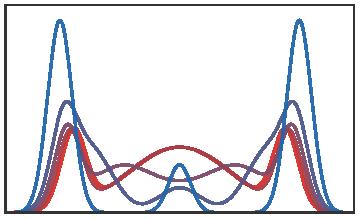
\includegraphics[width=.46\linewidth]{figures/kantorovich-wow-mixtures/component-level.pdf} &
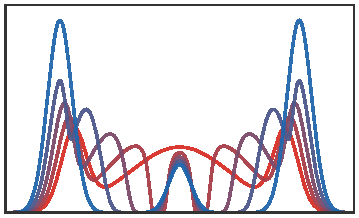
\includegraphics[width=.46\linewidth]{figures/kantorovich-wow-mixtures/collapsed-w2.pdf} \\[-.1em]
\small component law on Gaussian atoms &
\small collapsed mixture law
\index{collapsed mixture}% strictindex
\end{tabular}
\caption{\emph{Two interpolations between the same asymmetric three-component one-dimensional Gaussian mixtures.} The red endpoint has a broad central component carrying most of the mass, while the blue endpoint has two dominant sharp side modes. Left: Gaussian components are transported as atoms using their Bures-Wasserstein distance. Right: the collapsed densities are interpolated by the true one-dimensional quantile formula for $\Wass_2$. The central mass is split and recombined in the collapsed geometry, making the two paths visibly distinct.}
\index{Gaussian!mixture}% strictindex
\index{Wasserstein!distance}% strictindex
\index{quantile!formula}% strictindex
\label{fig:kantorovich-wow-mixtures}
\end{figure}

\begin{prop}[Collapsing is non-expansive]\label{prop-wow-collapsed-bound}
	Let $(\X,\dist)$ be Polish, let $1\leq p<\infty$, and let $\mathfrak A,\mathfrak B\in\Pp_p(\Pp_p(\X))$. For the collapsed mixtures defined by~\eqref{eq-wow-barycentric-mixture},
\index{barycentric!mixture}% strictindex
\index{collapsed mixture}% strictindex
	\[
		\Wass_p(\bar\alpha_{\mathfrak A},\bar\beta_{\mathfrak B})
		\leq
		\mathbb W_p(\mathfrak A,\mathfrak B).
	\]
\end{prop}
\begin{proof}
	Fix $\Pi\in\Couplings(\mathfrak A,\mathfrak B)$ and $\eta>0$. A standard measurable-selection theorem for optimal transport on Polish spaces gives a measurable kernel $(\alpha,\beta)\mapsto\pi_{\alpha,\beta}\in\Couplings(\alpha,\beta)$ such that
	\[
		\int_{\X\times\X}\dist(x,y)^p\,\d\pi_{\alpha,\beta}(x,y)
		\leq \Wass_p(\alpha,\beta)^p+\eta.
	\]
	Integrating this kernel against $\Pi$ gives a coupling $\bar\pi$ between $\bar\alpha_{\mathfrak A}$ and $\bar\beta_{\mathfrak B}$. Its cost satisfies
\index{measurable selection}% strictindex
\index{Markov kernel}% strictindex
\index{transport!cost}% strictindex
	\[
		\int_{\X\times\X}\dist(x,y)^p\d\bar\pi(x,y)
		\leq
		\int_{\Pp_p(\X)^2}\Wass_p^p(\alpha,\beta)\d\Pi(\alpha,\beta)+\eta.
	\]
	Letting $\eta\downarrow0$, taking the infimum over $\Pi$, and then taking the $p$-th root proves the claim.
\end{proof}

The following remark records a useful way in which this iterated construction reappears in the Gromov--Wasserstein lower bounds of the next section.

\begin{rem}[Local profiles as Wasserstein-over-Wasserstein laws]
	Given a metric-measure space $\XX=(\X,\dist_\X,\al_\X)$, each point defines a local distance distribution
\index{Wasserstein!distance}% strictindex
\index{Gromov-Wasserstein@Gromov--Wasserstein}% strictindex
\index{Gromov-Wasserstein@Gromov--Wasserstein!distance}% strictindex
\index{local distance distribution}% strictindex
\index{metric-measure space}% strictindex
\[
	\alpha_x=(\dist_\X(x,\cdot))_\sharp\al_\X\in\Pp(\RR_+),
	\qquad
	\mathfrak D_\XX=(x\mapsto\alpha_x)_\sharp\al_\X\in\Pp(\Pp(\RR_+)).
\]
The M\'emoli profile lower bound in Proposition~\ref{prop-memoli-gw-profile-lower-bound} is precisely a Wasserstein-over-Wasserstein comparison of these laws of local profiles. It replaces the full pairwise distortion by an ordinary OT problem whose ground cost is itself a one-dimensional Wasserstein distance.
\index{profile lower bound}% strictindex
\index{local profile}% strictindex
\index{distortion}% strictindex
\index{ground cost}% strictindex
\index{Memoli profile@M\'emoli profile}% strictindex
\index{Wasserstein!over Wasserstein}% strictindex
\index{Wasserstein!distance}% strictindex
%
\end{rem}

\section{Gromov--Wasserstein}
\index{Gromov-Wasserstein@Gromov--Wasserstein}% strictindex
\index{Gromov-Wasserstein@Gromov--Wasserstein!distance}% strictindex
\label{sec-gromov-wasserstein}

Gromov--Wasserstein compares spaces through their internal distance structures rather than through a fixed ambient ground cost. This is the right extension for graphs, shapes and point clouds whose points are not pre-aligned.
\index{ground cost}% strictindex

\paragraph{Discrete formulation.}

Optimal transport needs a ground cost $\C$ to compare histograms $(\a,\b)$, and thus cannot be used directly if the histograms are not defined on the same underlying space, or if one cannot pre-register these spaces to define a ground cost.
\index{histogram}% strictindex
%
To address this issue, one can instead use a weaker requirement: two matrices $\distD \in \RR^{n \times n}$ and $\distD' \in \RR^{m \times m}$ are available and represent relationships between the points on which the histograms are defined. A typical scenario is when these matrices are powers of distance matrices.
%
Define the quadratic distortion energy
\index{Gromov-Wasserstein@Gromov--Wasserstein}% strictindex
\begin{equation}\label{eq-gw-def}
\begin{aligned}
	\Ee_{\distD,\distD'}(\P)
	&\eqdef
	\sum_{i,j,i',j'} \De(\distD_{i,i'},\distD'_{j,j'})^p \P_{i,j}\P_{i',j'},
	\\
	\GWD( (\a,\distD), (\b,\distD') )^p
	&\eqdef
	\min_{\P \in \CouplingsD(\a,\b) }
	\Ee_{\distD,\distD'}(\P),
\end{aligned}
\end{equation}
where $p \geq 1$ and $\De$ is a distance on $\RR$, typically $\De(u,v)=|u-v|$.
%
The objective seeks a correspondence that is as close as possible to an isometry. Indeed, if two matched pairs $(i,j)$ and $(i',j')$ carry significant coupling mass, then their within-space distances should satisfy
\[
	\distD_{i,i'} \simeq \distD'_{j,j'}.
\]
Equivalently, $\Ee_{\distD,\distD'}(\P)$ is the expected distortion between two pairs drawn independently from $\P$. In the hard-assignment case $j=\sigma(i)$, minimizing it tries to enforce $\distD_{i,i'}\simeq\distD'_{\sigma(i),\sigma(i')}$ simultaneously for all pairs of matched points.
%
This is a quadratic optimization problem over the transport polytope, and its restriction to the feasible affine directions need not be convex. In the uniform case with the additional hard-assignment constraint $m=n$ and $\P$ a permutation matrix, the corresponding generalized structural-matching problem is a Quadratic Assignment Problem (QAP)~\cite{loiola-2007}. By contrast, for the relaxed finite-metric problem~\eqref{eq-gw-def}, neither NP-hardness nor a polynomial-time exact algorithm is currently known; the precise complexity status and references are given after~\eqref{eq-gw-zero-marginal-space}.
\index{assignment problem}% strictindex
\index{quadratic!assignment problem}% strictindex
\index{matrix!permutation}% strictindex
\index{transportation polytope}% strictindex
%
The relaxed coupling formulation used in GW can therefore be read as a soft graph-matching model~\cite{lyzinski-2015}.

\begin{example}[Application to structured objects]\label{ex-structured-objects-gw}
\index{structured data}% strictindex
\index{graph!matching}% strictindex
	Graphs, molecules, meshes and point clouds often do not come with a common coordinate system or a reliable node-to-node correspondence. GW compares them through their internal distances, so the coupling \(\P_{ij}\) becomes a soft structural correspondence rather than a spatial displacement. This is useful for graph matching, node embedding, shape comparison and molecule or mesh alignment~\cite{peyre2016gromov,vayer2019optimaltransportstructured}. When node attributes are also available, fused GW below adds a feature transport term to the intrinsic distortion, separating what should be preserved as structure from what should be matched as signal.
\end{example}

Figure~\ref{fig:gromov-isometry-matching} shows this intrinsic matching principle under progressively stronger deformations: correspondences are selected from within-space distance patterns rather than an ambient cross-space cost.

\begin{figure}[ht]
\centering
\begin{tabular}{@{}ccc@{}}
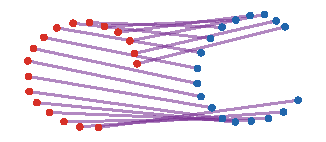
\includegraphics[width=.30\linewidth]{figures/gromov-isometry-matching/isometric.pdf} &
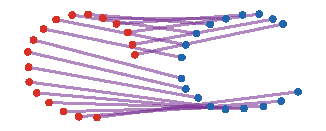
\includegraphics[width=.30\linewidth]{figures/gromov-isometry-matching/mild-deformation.pdf} &
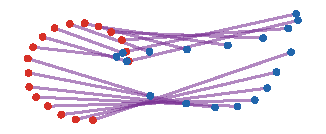
\includegraphics[width=.30\linewidth]{figures/gromov-isometry-matching/strong-deformation.pdf}
\\[-.1em]
\small isometric copy &
\small mild deformation &
\small strong deformation
\end{tabular}
\caption{\emph{Gromov--Wasserstein correspondences under increasing deformation.} The red and blue point clouds are not compared through an ambient Euclidean cross-cost; instead, the GW coupling compares their internal pairwise distances. A perfectly isometric copy admits a clean structural match, while mild and deliberately stronger deformations progressively bend the correspondence.}
\index{pairwise distance}% strictindex
\index{Gromov-Wasserstein@Gromov--Wasserstein}% strictindex
\index{correspondence}% strictindex
\label{fig:gromov-isometry-matching}
\end{figure}

When $\distD$ and $\distD'$ satisfy the metric axioms on $\{1,\ldots,m\}$ and $\{1,\ldots,n\}$, respectively, these weighted sets define finite metric-measure spaces with measures $\sum_i\a_i\delta_i$ and $\sum_j\b_j\delta_j$. Theorem~\ref{thm-gw-metric} therefore applies directly to~\eqref{eq-gw-def}: $\GWD$ satisfies the triangle inequality and defines a distance modulo measure-preserving isometries.
\index{triangle inequality}% strictindex
\index{measure-preserving!isometry}% strictindex
%
This distance was introduced and studied in detail by Memoli in~\cite{memoli-2011}. An in-depth mathematical exposition (in particular, its geodesic structure and gradient flows) is given in~\cite{SturmGW}. See also~\cite{schmitzer2013modelling} for applications in computer vision.
\index{gradient!flow}% strictindex
%
Its relation to Hausdorff and Gromov--Hausdorff distances is discussed at the end of this section.
\index{Hausdorff distance}% strictindex
\index{Gromov-Hausdorff distance}% strictindex

%%%%%%%%%%%%%%%%%%%%%
\paragraph{General setting.}

The continuous formulation abstracts the discrete distance matrices into metric-measure spaces, so that GW compares intrinsic geometries independently of labels, parametrizations or ambient coordinates.
\begin{defn}[Metric-measure space]\label{def-metric-measure-space}
\index{metric-measure space}% strictindex
	A metric-measure space is a triple
	\[
		\XX=(\X,\dist_\X,\al),
	\]
	where $(\X,\dist_\X)$ is Polish and $\al$ is a Borel probability measure on $\X$. For a finite $p$-Gromov--Wasserstein distance, one additionally assumes the finite-size condition
	\[
		\int_{\X\times\X}\dist_\X(x,x')^p\,\d\al(x)\d\al(x')<\infty.
	\]
\end{defn}
The general setting corresponds to computing couplings between metric-measure spaces $\XX=(\X,\dist_\X,\al)$ and $\YY=(\Y,\dist_\Y,\be)$, where the distance and the measure are both part of the data. Compactness is often assumed below to avoid additional tightness and integrability arguments.
%
The distortion between two metric-measure spaces is minimized over couplings of their mass distributions.
\begin{defn}[Gromov--Wasserstein distance]\label{def-gromov-wasserstein}
		Fix $p\geq1$ and a distance $\De$ on $[0,+\infty)$. Then
		\begin{align}
		\label{eq-gw-generic}
		\GW( \XX,\YY )^p \eqdef
		\umin{ \pi \in \Couplings(\al,\be) }
		\int_{\X^2 \times \Y^2}
		 \De(\dist_\X(x,x'),\dist_\Y(y,y'))^p
			 \d\pi(x,y)\d\pi(x',y').
		\end{align}
\end{defn}
Taking $\X=\{1,\ldots,m\}$, $\Y=\{1,\ldots,n\}$, $\al=\sum_i \a_i\delta_i$ and $\be=\sum_j \b_j\delta_j$ reduces~\eqref{eq-gw-generic} exactly to the discrete problem~\eqref{eq-gw-def}, since every coupling is represented by a matrix $\P\in\CouplingsD(\a,\b)$. Thus the construction above is precisely the finite-space, or equivalently finitely supported, specialization of the metric-measure formulation.

\paragraph{Comparison with Wasserstein and Wasserstein--Procrustes.}
The three distances retain different amounts of geometric information. Ordinary Wasserstein transport compares absolute positions, Wasserstein--Procrustes first removes ambient rigid motions, and GW retains only the metric-measure structure. On a common Euclidean ambient space, these nested invariances yield a useful two-sided estimate.

\begin{prop}[GW, Wasserstein--Procrustes and Wasserstein]\label{prop-gw-wasserstein-procrustes-comparison}\label{prop-gw-controlled-by-wasserstein}\label{prop-gw-procrustes-upper-certificate}
\index{probability measure}% strictindex
\index{Gromov-Wasserstein@Gromov--Wasserstein}% strictindex
\index{Wasserstein!distance}% strictindex
\index{Wasserstein!Procrustes}% strictindex
	Let $p\geq1$, let $\alpha,\beta\in\Pp_p(\X)$ be probability measures on the same metric space $(\X,\dist_\X)$, and take $\De(u,v)=|u-v|$ in~\eqref{eq-gw-generic}. Then
	\begin{equation}\label{eq-gw-fixed-space-wasserstein}
		\GW((\X,\dist_\X,\alpha),(\X,\dist_\X,\beta))
		\leq
		2\Wass_p(\alpha,\beta),
	\end{equation}
	where $\Wass_p$ uses the same ground metric $\dist_\X$. In particular, when $\X=\RR^d$ is equipped with the Euclidean distance, write $\XX_\alpha=(\RR^d,\norm{\cdot},\alpha)$ and $\XX_\beta=(\RR^d,\norm{\cdot},\beta)$. Then
	\begin{equation}\label{eq-gw-wp-wasserstein-comparison}
		\frac12\GW(\XX_\alpha,\XX_\beta)
		\leq
		\Wass_{p,\mathrm E(d)}([\alpha],[\beta])
		\leq
		\Wass_p(\alpha,\beta).
	\end{equation}
	For $p=2$, the middle term is the Wasserstein--Procrustes distance of Definition~\ref{def-wasserstein-procrustes}. The factor $1/2$ reflects the normalization in~\eqref{eq-gw-generic}; it disappears under the alternative convention $\De(u,v)=|u-v|/2$.
\end{prop}
\begin{proof}
	Fix $\pi\in\Couplings(\alpha,\beta)$, and draw $(x,y)$ and $(x',y')$ independently from $\pi$. The reverse triangle inequality gives
\index{triangle inequality}% strictindex
	\[
		\abs{\dist_\X(x,x')-\dist_\X(y,y')}
		\leq
		\dist_\X(x,y)+\dist_\X(x',y').
	\]
	Taking the $L^p(\pi\otimes\pi)$ norm, applying Minkowski's inequality, and optimizing over $\pi$ proves~\eqref{eq-gw-fixed-space-wasserstein}.

	Now specialize to $\RR^d$. Choosing the identity in Definition~\ref{def-quotient-wasserstein} proves the right inequality in~\eqref{eq-gw-wp-wasserstein-comparison}. Rigid motions preserve pairwise Euclidean distances, so the GW value is unchanged when $\alpha$ and $\beta$ are pushed forward by arbitrary $g,h\in\mathrm E(d)$. Applying~\eqref{eq-gw-fixed-space-wasserstein} to these aligned measures gives
	\[
		\GW(\XX_\alpha,\XX_\beta)
		\leq
		2\Wass_p(g_\sharp\alpha,h_\sharp\beta).
	\]
	Taking the infimum over $g,h$ proves the left inequality.
\index{Minkowski inequality}% strictindex
\end{proof}

To turn GW from a distortion score into a metric statement, one must quotient out the relabelings that preserve both distances and mass.

\begin{defn}[Isometric metric-measure spaces]\label{def-isometric-mm-spaces}
\index{metric-measure space}% strictindex
\index{measure-preserving!isometry}% strictindex
	Two metric-measure spaces $\XX=(\X,\dist_\X,\al)$ and $\YY=(\Y,\dist_\Y,\be)$ are isometric if there exists a bijection $\phi:\supp(\al)\to\supp(\be)$ such that $\phi_\sharp\al=\be$ and
	\[
		\dist_\Y(\phi(x),\phi(x'))=\dist_\X(x,x')
	\]
	for all $x,x'\in\supp(\al)$.
\end{defn}

The next theorem explains why the averaged distortion above is not merely a matching score. Once one quotients out measure-preserving isometries, it defines a genuine distance between metric-measure spaces.
\index{distortion}% strictindex
\index{measure-preserving!isometry}% strictindex
\index{metric-measure space}% strictindex

\begin{thm}[Gromov--Wasserstein metric modulo isometries]\label{thm-gw-metric}
\index{Gromov-Wasserstein@Gromov--Wasserstein}% strictindex
\index{Gromov-Wasserstein@Gromov--Wasserstein!metric}% strictindex
\index{modulo isometry}% strictindex
	For compact metric-measure spaces, $p\geq1$ and $\De(u,v)=|u-v|$, $\GW$ defines a distance up to measure-preserving isometries.
\end{thm}

\begin{proof}
	Compactness of the supports makes the coupling set compact and the distortion functional continuous, so an optimal coupling exists. If $\phi$ is a measure-preserving isometry, the graph coupling $(\Id,\phi)_\sharp\al$ has zero distortion; in particular, $\GW(\XX,\XX)=0$. Symmetry and non-negativity are immediate.

	If $\GW(\XX,\YY)=0$ and $\pi$ is an optimal plan, then $\dist_\X(x,x')=\dist_\Y(y,y')$ holds $\pi\otimes\pi$-almost everywhere. By continuity, this equality holds on $\supp(\pi)^2$. We show that $\XX$ and $\YY$ are isometric by showing that both are isometric to the support space $(\supp(\pi),\dist_\pi,\pi)$, where
\index{optimal plan}% strictindex
	\[
		\dist_\pi((x,y),(x',y'))
		\eqdef
		\frac12\dist_\X(x,x')+\frac12\dist_\Y(y,y').
	\]
	The first projection $\psi:(x,y)\mapsto x$ is measure-preserving. For $((x,y),(x',y'))\in\supp(\pi)^2$,
	\[
		\dist_\X(\psi(x,y),\psi(x',y'))
		=
		\dist_\X(x,x')
		=
		\dist_\Y(y,y')
		=
		\dist_\pi((x,y),(x',y')),
	\]
	so $\psi$ is an isometry and therefore injective. To see surjectivity onto $\supp(\al)$, take $x\in\supp(\al)$. Since $\psi_\sharp\pi=\al$, there is a sequence $(x_k,y_k)\in\supp(\pi)$ with $x_k\to x$. The equality of distances on $\supp(\pi)$ makes $(y_k)_k$ Cauchy, and compactness gives a convergent subsequence with limit $(x,y)\in\supp(\pi)$. The same argument for the second projection shows that the support space is also isometric to $\YY$.

	For the triangle inequality, let $\pi$ be an optimal coupling between $\XX$ and $\YY$, and $\xi$ an optimal coupling between $\YY$ and $\ZZ=(\Z,\dist_\Z,\ga)$. By the gluing lemma, take $\sigma$ on $\X\times\Y\times\Z$ whose $(\X,\Y)$ and $(\Y,\Z)$ marginals are $\pi$ and $\xi$. Let $\rho=(P_{\X,\Z})_\sharp\sigma$, and write $\bar\sigma=\sigma\otimes\sigma$ for the product law of two independent triples $(x,y,z)$ and $(x',y',z')$. Then $\rho$ is feasible between $\XX$ and $\ZZ$, and
\index{triangle inequality}% strictindex
\index{optimal coupling}% strictindex
\index{gluing lemma}% strictindex
	\begin{align*}
		\GW(\XX,\ZZ)
		&\leq
		\left(
		\int
		\abs{\dist_\X(x,x')-\dist_\Z(z,z')}^p
		\d\bar\sigma
		\right)^{1/p} \\
		&\leq
		\left(
		\int
		\abs{\dist_\X(x,x')-\dist_\Y(y,y')}^p
		\d\bar\sigma
		\right)^{1/p}
		+
		\left(
		\int
		\abs{\dist_\Y(y,y')-\dist_\Z(z,z')}^p
		\d\bar\sigma
		\right)^{1/p} \\
		&=
		\GW(\XX,\YY)+\GW(\YY,\ZZ),
	\end{align*}
	where the second inequality uses the pointwise triangle inequality followed by Minkowski's inequality. This proves the triangle inequality and completes the metric proof.
\index{Minkowski inequality}% strictindex
\end{proof}

\begin{rem}[Distance hierarchy and topology]\label{rem-gw-wp-topologies}
The comparison~\eqref{eq-gw-wp-wasserstein-comparison} immediately gives
\[
	\Wass_p\text{-convergence}
	\quad\Longrightarrow\quad
	\Wass_{p,\mathrm E(d)}\text{-convergence}
	\quad\Longrightarrow\quad
	\GW\text{-convergence}.
\]
The first implication is strict when measures, rather than their rigid-motion orbits, are compared. For example, let $\alpha=\tfrac23\delta_0+\tfrac13\delta_{e_1}$ and $\alpha_n=(x\mapsto x+ne_1)_\sharp\alpha$. Then $\Wass_{p,\mathrm E(d)}([\alpha_n],[\alpha])=\GW(\XX_{\alpha_n},\XX_\alpha)=0$ for every $n$, whereas $\Wass_p(\alpha_n,\alpha)=n$. Thus rigid registration removes a genuine obstruction to ordinary Wasserstein convergence.

The second implication is subtler. On families of compact Euclidean metric-measure spaces with fixed ambient dimension and uniformly bounded diameters, there is no sequence that converges in GW but not in Wasserstein--Procrustes. Indeed, a distance-preserving bijection between Euclidean supports extends from their affine hulls to an ambient rigid motion, so the two distances have the same zero classes. More quantitatively, M\'emoli~\cite{memoli-2011} proves that distortion GW and Sturm's common-embedding transport distance induce the same topology, while~\cite{memoli-2008} gives a dimension-dependent H\"older comparison between the latter and isometry-invariant Wasserstein transport on uniformly bounded Euclidean sets. Consequently, GW and Wasserstein--Procrustes induce the same quotient topology on this class, although they are not uniformly Lipschitz equivalent. Thus the three distances are genuinely different numerically, but they do not define three strictly nested topologies in this Euclidean setting.
\end{rem}

\paragraph{Marginal stability and geodesics.}
The GW metric structure controls changes in the marginal measures and also provides intrinsic displacement interpolations between metric-measure spaces.

A useful consequence is that, when the geometry is fixed and only the sampling of the measures changes, GW inherits ordinary Wasserstein sampling rates. This is often the right way to read empirical GW: the non-convexity of the coupling problem is algorithmic, but the value is Lipschitz with respect to marginal perturbations measured in $\Wass_p$.
\index{sample complexity}% strictindex
\index{empirical!measure}% strictindex
\index{Gromov-Wasserstein@Gromov--Wasserstein!sample complexity}% strictindex

\begin{prop}[Marginal stability and empirical GW rates]\label{prop-gw-empirical-stability}
\index{Gromov-Wasserstein@Gromov--Wasserstein!sample complexity}% strictindex
	Let $\XX=(\X,\dist_\X,\alpha)$ and $\YY=(\Y,\dist_\Y,\beta)$ be compact metric-measure spaces, with $\De(u,v)=|u-v|$ and exponent $p\geq1$. For any probability measures $\tilde\alpha$ on $\X$ and $\tilde\beta$ on $\Y$, set
	\[
		\widetilde\XX=(\X,\dist_\X,\tilde\alpha),
		\qquad
		\widetilde\YY=(\Y,\dist_\Y,\tilde\beta).
	\]
	Then, deterministically,
	\[
		\abs{\GW(\widetilde\XX,\widetilde\YY)-\GW(\XX,\YY)}
		\leq
		2\Wass_p^\X(\tilde\alpha,\alpha)
		+
		2\Wass_p^\Y(\tilde\beta,\beta),
	\]
	where $\Wass_p^\X$ and $\Wass_p^\Y$ denote Wasserstein distances computed with $\dist_\X$ and $\dist_\Y$. If $\hat\alpha_n$ and $\hat\beta_m$ are independent empirical measures built from iid samples with laws $\alpha$ and $\beta$, write $\widehat\XX_n=(\X,\dist_\X,\hat\alpha_n)$ and $\widehat\YY_m=(\Y,\dist_\Y,\hat\beta_m)$.
	If, in addition, $\X$ and $\Y$ are regular compact subsets of Euclidean spaces of intrinsic dimensions $d_\X$ and $d_\Y$, and the high-dimensional Wasserstein regime $d_\X,d_\Y>2p$ applies, then
	\[
		\EE\abs{\GW(\widehat\XX_n,\widehat\YY_m)-\GW(\XX,\YY)}
		=
		O(n^{-1/d_\X}+m^{-1/d_\Y}).
	\]
	For $p=1$ on subsets of $[0,1]^d$, the rates, including the low-dimensional logarithmic cases, are those of Proposition~\ref{prop-empirical-ot-rate}.
\end{prop}

\begin{proof}
	The triangle inequality of Theorem~\ref{thm-gw-metric} gives
	\[
		\GW(\widetilde\XX,\widetilde\YY)
		-
		\GW(\XX,\YY)
		\leq
		\GW(\widetilde\XX,\XX)
		+
		\GW(\YY,\widetilde\YY).
	\]
	Exchanging the two pairs gives the same bound for the opposite difference, hence the absolute value. The two terms on the right compare metric-measure spaces with the same underlying metric and only different measures, so Proposition~\ref{prop-gw-controlled-by-wasserstein} bounds them by $2\Wass_p^\X(\tilde\alpha,\alpha)$ and $2\Wass_p^\Y(\tilde\beta,\beta)$. Substituting $\tilde\alpha=\hat\alpha_n$ and $\tilde\beta=\hat\beta_m$, taking expectations and applying the empirical Wasserstein rates recalled in Section~\ref{sec-sample-complexity} gives the stated Euclidean rate.
\index{triangle inequality}% strictindex
\index{empirical!OT rate}% strictindex
\end{proof}

The metric structure also gives geodesics. Sturm's construction is useful conceptually because it makes it possible to discuss interpolation, barycenters and gradient flows directly on the space of metric-measure spaces, even though the intermediate space lives on a product support and is therefore expensive numerically~\cite{SturmGW}.
\index{metric-measure space}% strictindex
\index{gradient!flow}% strictindex

\begin{prop}[Gromov--Wasserstein geodesics]\label{prop-gw-geodesics}
\index{Wasserstein!geodesic}% strictindex
\index{Gromov-Wasserstein@Gromov--Wasserstein}% strictindex
\index{Gromov-Wasserstein@Gromov--Wasserstein!geodesic}% strictindex
	Let $\XX_0=(\X_0,\dist_{\X_0},\al_0)$ and $\XX_1=(\X_1,\dist_{\X_1},\al_1)$ be compact metric-measure spaces, take $\De(u,v)=|u-v|$ in~\eqref{eq-gw-generic}, and let $\pi^\star$ be an optimal coupling. Define, on $\Z=\X_0\times\X_1$,
\index{optimal coupling}% strictindex
	\[
		\dist_t((x_0,x_1),(x'_0,x'_1))
		\eqdef
		(1-t)\dist_{\X_0}(x_0,x'_0)+t\dist_{\X_1}(x_1,x'_1),
		\qquad
		\XX_t=(\Z,\dist_t,\pi^\star).
	\]
	For $0<t<1$, $\dist_t$ is a metric. At $t=0$ and $t=1$, one quotients $\Z$ by the zero-distance relation associated with $\dist_t$. Then $t\mapsto\XX_t$ is a constant-speed geodesic:
\index{constant-speed geodesic}% strictindex
	\[
		\GW(\XX_s,\XX_t)=|t-s|\GW(\XX_0,\XX_1)
		\qquad
		\forall s,t\in[0,1].
	\]
\end{prop}

\begin{proof}
	Write $D=\GW(\XX_0,\XX_1)$. For $s<t$, couple $\XX_s$ and $\XX_t$ by the diagonal coupling induced by the identity on $\Z$ and the measure $\pi^\star$. For two independent points $z=(x_0,x_1)$ and $z'=(x'_0,x'_1)$ sampled from $\pi^\star$,
	\[
		\dist_t(z,z')-\dist_s(z,z')
		=
		(t-s)\big(\dist_{\X_1}(x_1,x'_1)-\dist_{\X_0}(x_0,x'_0)\big).
	\]
	Using this feasible coupling gives $\GW(\XX_s,\XX_t)\leq(t-s)D$. The same construction with the projections from $\Z$ to $\X_0$ and $\X_1$ gives $\GW(\XX_0,\XX_t)\leq tD$ and $\GW(\XX_t,\XX_1)\leq(1-t)D$. The triangle inequality for $\GW$ then yields, for $0\leq s\leq t\leq1$,
\index{triangle inequality}% strictindex
\index{feasible coupling}% strictindex
	\[
		D
		\leq
		\GW(\XX_0,\XX_s)+\GW(\XX_s,\XX_t)+\GW(\XX_t,\XX_1)
		\leq
		sD+\GW(\XX_s,\XX_t)+(1-t)D,
	\]
	so $\GW(\XX_s,\XX_t)\geq(t-s)D$. This proves equality.
\end{proof}

Figure~\ref{fig:gromov-nonisometric-distortion} complements the global GW objective with local diagnostics, displaying where a mildly non-isometric correspondence creates the largest pairwise-distance residuals.

\begin{figure}[ht]
\centering
\begin{tabular}{@{}cc@{}}
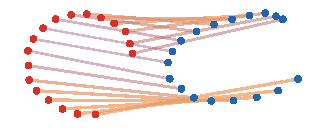
\includegraphics[width=.43\linewidth]{figures/gromov-nonisometric-distortion/correspondence.pdf} &
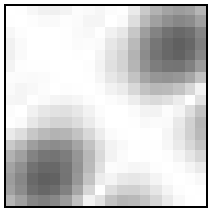
\includegraphics[width=.23\linewidth]{figures/gromov-nonisometric-distortion/distance-residual.pdf}
\\[-.1em]
\small hard correspondence $\sigma$ &
\small residual $|d_\X-d_\Y\circ\sigma|$
\end{tabular}
\caption{\emph{Local distortion in a mildly non-isometric GW match.} The left panel colors transport segments by the average residual induced by the displayed hard correspondence. The right panel shows the pairwise-distance residual matrix $|d_\X(x_i,x_{i'})-d_\Y(y_{\sigma(i)},y_{\sigma(i')})|$ in white-to-black scale, with darker entries marking larger local distortion. This matrix is the local contribution minimized by the discrete GW objective for the displayed correspondence.}
\index{distance residual}% strictindex
\index{distortion}% strictindex
\index{correspondence}% strictindex
\label{fig:gromov-nonisometric-distortion}
\end{figure}

\paragraph{Distance-profile lower bound.}
Local distance distributions provide an inexpensive intrinsic certificate and a useful initialization principle for the non-convex solver.
\index{profile lower bound}% strictindex

\begin{prop}[M\'emoli profile lower bound]\label{prop-memoli-gw-profile-lower-bound}
\index{Memoli profile@M\'emoli profile}% strictindex
	Let $\XX=(\X,\dist_\X,\alpha)$ and $\YY=(\Y,\dist_\Y,\beta)$ be compact metric-measure spaces and take $\De(u,v)=|u-v|$ in~\eqref{eq-gw-generic}, with the same exponent $p\geq1$. For each $x\in\X$ and $y\in\Y$, define the distance-profile measures on $\RR_+$ by
\index{metric-measure space}% strictindex
	\[
		\alpha_x\eqdef(\dist_\X(x,\cdot))_\sharp\alpha,
		\qquad
		\beta_y\eqdef(\dist_\Y(y,\cdot))_\sharp\beta.
	\]
	Let $\mathfrak D_\XX=(x\mapsto\alpha_x)_\sharp\alpha$ and $\mathfrak D_\YY=(y\mapsto\beta_y)_\sharp\beta$, which are probability measures on $\Pp_p(\RR_+)$. Then
\index{probability measure}% strictindex
	\[
		\mathbb W_p\bigl(\mathfrak D_\XX,\mathfrak D_\YY\bigr)
		\leq
		\GW(\XX,\YY).
	\]
	Here $\mathbb W_p$ is the Wasserstein-over-Wasserstein distance~\eqref{eq-wow-distance}: its ground space is $(\Pp_p(\RR_+),\Wass_p)$.
\index{ground cost}% strictindex
\index{Wasserstein!distance}% strictindex
\end{prop}
\begin{proof}
	Fix any $\pi\in\Couplings(\alpha,\beta)$. It induces a coupling $(x,y)\mapsto(\alpha_x,\beta_y)$ between $\mathfrak D_\XX$ and $\mathfrak D_\YY$, hence
	\[
		\mathbb W_p\bigl(\mathfrak D_\XX,\mathfrak D_\YY\bigr)^p
		\leq
		\int_{\X\times\Y}\Wass_p(\alpha_x,\beta_y)^p\,\d\pi(x,y).
	\]
	For fixed $(x,y)$, the map $(x',y')\mapsto(\dist_\X(x,x'),\dist_\Y(y,y'))$ pushes the same coupling $\pi$ to a coupling between $\alpha_x$ and $\beta_y$. Therefore
	\[
		\Wass_p(\alpha_x,\beta_y)^p
		\leq
		\int_{\X\times\Y}
		\abs{\dist_\X(x,x')-\dist_\Y(y,y')}^p
		\d\pi(x',y').
	\]
	Integrating in $(x,y)$ gives
	\[
		\mathbb W_p\bigl(\mathfrak D_\XX,\mathfrak D_\YY\bigr)^p
		\leq
		\int_{\X^2\times\Y^2}
		\abs{\dist_\X(x,x')-\dist_\Y(y,y')}^p
		\d\pi(x,y)\d\pi(x',y').
	\]
	Taking the infimum over $\pi$ and then the $p$-th root proves the claim.
\end{proof}

Figure~\ref{fig:gromov-memoli-distance-profiles} makes the two transport levels explicit for the planar shapes $\XX$ and $\YY$: sorting each distance profile computes the one-dimensional costs, then an outer assignment couples the resulting profile laws.

\begin{figure}[ht]
\centering
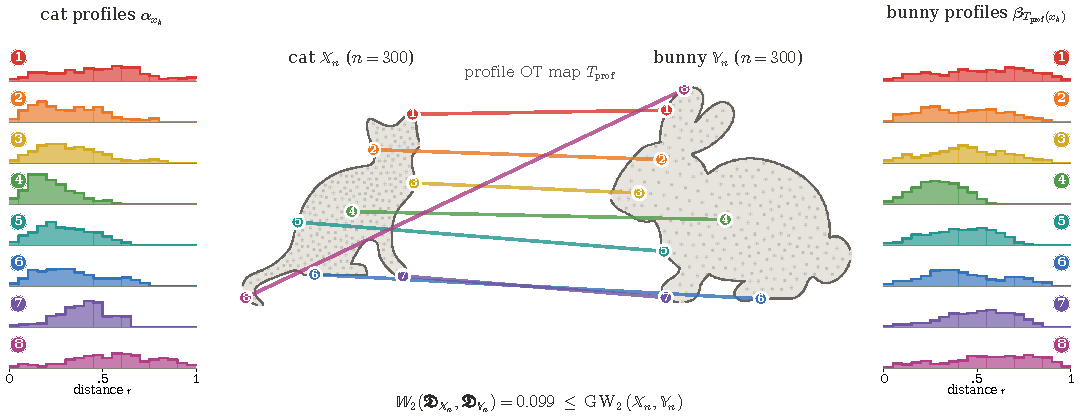
\includegraphics[width=.99\linewidth]{figures/gromov-memoli-distance-profiles/profiles.pdf}
\caption{\emph{M\'emoli distance profiles expose a computable lower bound for intrinsic GW comparison.} The planar shapes $\XX$ and $\YY$ are represented by cat and bunny silhouettes, centered and normalized to unit diameter. Matching colors identify representative anchor pairs selected by the optimal assignment for the profile cost $\C_{ij}=\Wass_2^2(\alpha_{x_i},\beta_{y_j})$, their connecting segments, and the corresponding distance-profile histograms in the side columns. The histograms are display summaries only: the profile costs are computed by sorting the complete distance profiles. The resulting outer assignment realizes the M\'emoli profile lower bound.}
\label{fig:gromov-memoli-distance-profiles}
\index{Memoli profile@M\'emoli profile}% strictindex
\index{distance profile}% strictindex
\index{Wasserstein!over Wasserstein}% strictindex
\end{figure}

This lower bound is useful computationally because the profile cost matrix $\C_{ij}=\Wass_p(\alpha_{x_i},\beta_{y_j})^p$ is an ordinary OT cost between points. Solving this easier OT problem gives a geometry-aware initialization for the non-convex GW iterations below, before the full pairwise-distance distortion is optimized.

The profile lower bound is intrinsic. In Euclidean applications, Proposition~\ref{prop-gw-wasserstein-procrustes-comparison} pairs it with an extrinsic upper certificate obtained by registering the measures before applying ordinary Wasserstein transport. Combining the two propositions gives the extended Euclidean sandwich
\index{Wasserstein!Procrustes}% strictindex
\begin{equation}\label{eq-gw-profile-procrustes-sandwich}
\mathbb W_p(\mathfrak D_\XX,\mathfrak D_\YY)
\leq
\GW(\XX,\YY)
\leq
2\,\Wass_{p,\mathrm E(d)}([\alpha],[\beta])
\leq
2\,\Wass_p(\alpha,\beta),
\end{equation}
where $\XX=(\RR^d,\norm{\cdot},\alpha)$ and $\YY=(\RR^d,\norm{\cdot},\beta)$. The profile term is an inexpensive intrinsic certificate, while the Wasserstein--Procrustes term gives an extrinsic certificate after optimal rigid registration. The final inequality simply omits registration and is therefore generally looser.
\index{distortion}% strictindex
\index{cost!matrix}% strictindex
\index{Wasserstein!Procrustes}% strictindex

\paragraph{GW as a concave minimization problem.}
Unlike linear OT, GW minimizes a quadratic functional over the convex set of couplings. Its first-order linearization is nevertheless an ordinary OT problem, which provides the basic stationarity condition used by essentially all GW solvers. The limitation is fundamental: solving this self-consistent linearized problem is necessary at a local minimum, but does not by itself certify either local or global optimality.
\index{Gromov-Wasserstein@Gromov--Wasserstein!conditional concavity}% strictindex
\index{quadratic!form}% strictindex
\index{concave!minimization}% strictindex
\index{conditionally negative definite kernel}% strictindex
\index{stationary point}% strictindex

To isolate the relevant curvature, set $\mathcal Z=\X\times\Y$ and
\[
	L\bigl((x,y),(x',y')\bigr)
	\eqdef
	\De\bigl(\dist_\X(x,x'),\dist_\Y(y,y')\bigr)^p.
\]
For finite signed measures $\xi,\eta\in\Mm(\mathcal Z)$ for which the integrals are absolutely convergent, define the symmetric bilinear form and its associated quadratic form by
\begin{equation}\label{eq-gw-quadratic-form}
	\mathcal B_L(\xi,\eta)
	\eqdef
	\iint_{\mathcal Z^2}L(z,z')\d\xi(z)\d\eta(z'),
	\qquad
	\mathcal Q_L(\xi)
	\eqdef\mathcal B_L(\xi,\xi).
\end{equation}
Thus~\eqref{eq-gw-generic} minimizes $\mathcal Q_L(\pi)$ over $\pi\in\Couplings(\alpha,\beta)$. At a coupling $\pi$, define the linearized ground cost
\begin{equation}\label{eq-gw-linearized-cost}
	c_\pi(z)
	\eqdef
	2\int_{\mathcal Z}L(z,z')\d\pi(z').
\end{equation}
For any $\widehat\pi\in\Couplings(\alpha,\beta)$ and $\xi=\widehat\pi-\pi$, the exact quadratic expansion is
\begin{equation}\label{eq-gw-exact-linearization}
	\mathcal Q_L(\pi+t\xi)
	=
	\mathcal Q_L(\pi)
	{}+t\int_{\mathcal Z}c_\pi\d\xi
	{}+t^2\mathcal Q_L(\xi).
\end{equation}

\begin{defn}[First-order stationary GW coupling]\label{def-gw-stationary-coupling}
	A coupling $\pi\in\Couplings(\alpha,\beta)$ is \emph{first-order stationary for GW} if it satisfies the variational inequality
	\begin{equation}\label{eq-gw-stationary-variational-inequality}
		\int_{\mathcal Z}c_\pi\d(\widehat\pi-\pi)\geq0
		\qquad\text{for every }\widehat\pi\in\Couplings(\alpha,\beta).
	\end{equation}
\end{defn}
This is stationarity for constrained minimization, not the unconstrained equation $c_\pi=0$: in finite dimensions it is the usual variational inequality $-\nabla\mathcal Q_L(\pi)\in N_{\Couplings(\alpha,\beta)}(\pi)$, with the normal-cone convention $N_K(x)=\{q:\langle q,y-x\rangle\leq0\ \forall y\in K\}$.

\begin{prop}[Frozen-OT characterization of stationarity]\label{prop-gw-frozen-ot-stationarity}
	A coupling $\pi$ is first-order stationary in the sense of Definition~\ref{def-gw-stationary-coupling} if and only if
	\begin{equation}\label{eq-gw-frozen-ot-fixed-point}
		\pi\in\argmin_{\widehat\pi\in\Couplings(\alpha,\beta)}
		\int_{\mathcal Z}c_\pi\d\widehat\pi.
	\end{equation}
	In particular, every local minimizer for the narrow topology, and hence every global minimizer, of $\mathcal Q_L$ is an optimal Kantorovich coupling for its own linearized cost $c_\pi$.
\end{prop}
\begin{proof}
	The variational inequality~\eqref{eq-gw-stationary-variational-inequality} is exactly the assertion that $\pi$ minimizes the linear functional $\widehat\pi\mapsto\int c_\pi\d\widehat\pi$, proving the equivalence. If $\pi$ is a local minimizer and $\widehat\pi$ is arbitrary, the segment $\pi_t=(1-t)\pi+t\widehat\pi$ remains feasible. The right derivative at $t=0$ in~\eqref{eq-gw-exact-linearization} must be nonnegative, which gives~\eqref{eq-gw-stationary-variational-inequality}.
\end{proof}

The converse is false: frozen-OT self-consistency is only a first-order condition. Even the concave quadratic $q(s)=-s^2$ on $[-1,1]$ has the stationary point $s=0$, which is a strict maximum rather than a minimum. Conditional concavity therefore does not turn arbitrary stationary couplings into global minimizers. What it does provide is a global upper model for the objective, a monotone linearization step, and a replacement principle for the frozen problem at a global minimizer. These are substantially stronger conclusions than are available for a generic non-convex quadratic program.

To formulate this additional structure, introduce the linear marginalization operator and its kernel
\begin{equation}\label{eq-gw-zero-marginal-space}
	\begin{aligned}
	\operatorname{Marg}_{\X,\Y}:\Mm(\X\times\Y)
	&\longrightarrow\Mm(\X)\times\Mm(\Y),\\
	\xi
	&\longmapsto\bigl((P_\X)_\sharp\xi,(P_\Y)_\sharp\xi\bigr),\\
	\mathcal T_{\X,\Y}
	&\eqdef
	\ker\bigl(\operatorname{Marg}_{\X,\Y}\bigr)
	=
	\enscond{\xi\in\Mm(\X\times\Y)}{(P_\X)_\sharp\xi=0,\ (P_\Y)_\sharp\xi=0}.
	\end{aligned}
\end{equation}
The space $\mathcal T_{\X,\Y}$ depends only on the two ambient spaces, not on the values of $\alpha$ and $\beta$: it is the direction space parallel to the affine marginal constraints. Every difference of two feasible couplings belongs to it. For finite spaces, identifying $\xi$ with an $m\times n$ matrix $\Xi$ gives
\[
	\mathcal T_{\X,\Y}
	=
	\enscond{\Xi\in\RR^{m\times n}}{\Xi\ones_n=0,\ \transp{\Xi}\ones_m=0},
	\qquad
	\dim\mathcal T_{\X,\Y}=(m-1)(n-1).
\]
When the marginals are positive, this is exactly the translation space of the affine hull of the transport polytope. Along any segment $\pi_t=\pi+t\xi$ that remains feasible on an interval, one has
\[
	\frac{\mathrm d^2}{\mathrm dt^2}\mathcal Q_L(\pi_t)=2\mathcal Q_L(\xi).
\]
Thus positivity of the ambient kernel $L$ is not the right question. Along a feasible segment, convexity is controlled by the sign of $\mathcal Q_L$ on its zero-marginal direction. In finite spaces with positive marginals, every element of $\mathcal T_{\X,\Y}$ generates a sufficiently short feasible segment, so convexity on the transport polytope is equivalent to $\mathcal Q_L(\xi)\geq0$ for every $\xi\in\mathcal T_{\X,\Y}$. No such sign can be expected for a general GW loss.

The regime studied next has the opposite sign, $\mathcal Q_L(\xi)\leq0$ on zero-marginal directions, and hence makes $\mathcal Q_L$ concave on the coupling set. Minimizing a concave function remains a genuinely non-convex problem and tends to push solutions toward the combinatorial boundary of the transport polytope. Concave quadratic minimization over polytopes is NP-hard in general: on the Birkhoff polytope, one may subtract a sufficiently large multiple of $\norm{\P}_{\mathrm F}^2$ from a QAP objective to make it concave; this term is constant on permutation matrices, and a concave minimum is attained at an extreme point~\cite{loiola-2007}. Concavity should therefore be read as exploitable structure rather than tractability.

This generic hardness statement must not be over-specialized: it does not prove that relaxed GW between finite metric spaces is NP-hard. The revised analysis in~\cite{Kravtsova2024GWComplexity} proves that the ambient quadratic coefficient matrix is not positive semidefinite for nontrivial finite metric instances, but explicitly notes that no reduction from a known NP-hard problem is currently available for the relaxed metric problem. Conversely, no general polynomial-time exact algorithm is known. Exact relaxed metric GW should therefore be described, in general, as a non-convex quadratic problem of unresolved worst-case complexity, rather than as a problem with an established NP-hardness theorem; practical algorithms typically target stationary points.
\index{Gromov-Monge@Gromov--Monge}% strictindex
\index{quadratic!assignment problem}% strictindex
\index{computational complexity}% strictindex

The next result identifies a broad regime in which the sign of the quadratic form is known on the only directions that matter. Recall the conditionally positive and conditionally negative kernels of Definition~\ref{def-positive-kernels}.

\begin{prop}[Conditional concavity of squared GW]\label{prop-gw-conditional-concavity}
	Let $\X$ and $\Y$ be compact metric spaces, and let $\alpha\in\Mm_+^1(\X)$ and $\beta\in\Mm_+^1(\Y)$. In~\eqref{eq-gw-generic}, take $p=2$ and $\De(u,v)=|u-v|$. Assume that the two distance kernels $\dist_\X$ and $\dist_\Y$ are either both conditionally positive definite or both conditionally negative definite in the sense of Definition~\ref{def-positive-kernels}. Then
	\begin{equation}\label{eq-gw-conditional-negative-form}
		\mathcal Q_L(\xi)\leq0
		\qquad\text{for every }\xi\in\mathcal T_{\X,\Y}.
	\end{equation}
	Consequently, $\pi\mapsto\mathcal Q_L(\pi)$ is concave on $\Couplings(\alpha,\beta)$.
\end{prop}
\begin{proof}
	The zero marginal conditions make the two pure terms in the squared loss vanish, and therefore
	\[
		\mathcal Q_L(\xi)
		=
		-2\iint \dist_\X(x,x')\dist_\Y(y,y')\d\xi(x,y)\d\xi(x',y').
	\]
	Choose $s\in\{-1,1\}$ so that $s\dist_\X$ and $s\dist_\Y$ are conditionally positive definite. Fix base points $x_0\in\X$ and $y_0\in\Y$, and define the centered kernels
	\begin{align*}
		\widetilde{\dist}_\X(x,x')
		&=s\bigl(\dist_\X(x,x')-\dist_\X(x,x_0)-\dist_\X(x_0,x')+\dist_\X(x_0,x_0)\bigr),\\
		\widetilde{\dist}_\Y(y,y')
		&=s\bigl(\dist_\Y(y,y')-\dist_\Y(y,y_0)-\dist_\Y(y_0,y')+\dist_\Y(y_0,y_0)\bigr).
	\end{align*}
	These kernels are positive definite. Since $\xi$ has zero marginals and $s^2=1$, every centering term vanishes after integration. Let $\Phi_\X$ and $\Phi_\Y$ be Hilbert feature maps for $\widetilde{\dist}_\X$ and $\widetilde{\dist}_\Y$. Compactness and continuity make these maps bounded. Writing $z=(x,y)$ and $z'=(x',y')$, one obtains
	\[
		\iint_{\mathcal Z^2}\dist_\X(x,x')\dist_\Y(y,y')\d\xi(z)\d\xi(z')
		=
		\norm{\int_{\mathcal Z}\Phi_\X(x)\otimes\Phi_\Y(y)\d\xi(z)}^2
		\geq0.
	\]
	This proves~\eqref{eq-gw-conditional-negative-form}; the second-derivative identity above then proves concavity on every feasible segment.
\end{proof}

The sign condition partially closes the gap between a quadratic GW problem and its frozen linearization. It does not make stationarity sufficient, but it makes the tangent model a global majorizer and allows any frozen optimizer at a known global solution to replace that solution without changing the GW value.

\begin{prop}[Tangent majorization and frozen-OT replacement]\label{prop-gw-frozen-ot-replacement}
	Assume that $\mathcal Q_L$ is concave on $\Couplings(\alpha,\beta)$. Then, for every $\pi,\widehat\pi\in\Couplings(\alpha,\beta)$,
	\begin{equation}\label{eq-gw-tangent-majorization}
		\mathcal Q_L(\widehat\pi)
		\leq
		\mathcal Q_L(\pi)
		+
		\int_{\mathcal Z}c_\pi\d(\widehat\pi-\pi)
		=
		2\mathcal B_L(\pi,\widehat\pi)-\mathcal Q_L(\pi).
	\end{equation}
	Consequently:
	\begin{enumerate}
		\item if $\pi^+\in\argmin_{\eta\in\Couplings(\alpha,\beta)}\int c_\pi\d\eta$, then $\mathcal Q_L(\pi^+)\leq\mathcal Q_L(\pi)$;
		\item if $\pi_\star$ is globally GW-optimal, then every minimizer of the frozen OT problem with cost $c_{\pi_\star}$ is also globally GW-optimal.
	\end{enumerate}
\end{prop}
\begin{proof}
	Apply~\eqref{eq-gw-exact-linearization} at $t=1$ with $\xi=\widehat\pi-\pi$. Concavity gives $\mathcal Q_L(\xi)\leq0$, which proves~\eqref{eq-gw-tangent-majorization}. For the first conclusion, frozen optimality gives $\int c_\pi\d(\pi^+-\pi)\leq0$. For the second, Proposition~\ref{prop-gw-frozen-ot-stationarity} shows that $\pi_\star$ itself minimizes its frozen objective. Hence any other frozen minimizer $\widehat\pi$ satisfies $\int c_{\pi_\star}\d(\widehat\pi-\pi_\star)=0$, and~\eqref{eq-gw-tangent-majorization} gives $\mathcal Q_L(\widehat\pi)\leq\mathcal Q_L(\pi_\star)$. Global minimality gives the reverse inequality.
\end{proof}

Thus freezing one occurrence of the coupling produces a global upper bound, not merely a formal linearization. The second conclusion is a replacement theorem, not a characterization of global minimizers: a generic stationary point can still be a maximum or a non-global local minimum.

Schoenberg's theorem gives the principal Euclidean example: on compact subsets of Euclidean spaces, $\dist_\X(x,x')=\norm{x-x'}^q$ and $\dist_\Y(y,y')=\norm{y-y'}^q$ are conditionally negative definite for $0<q\leq2$~\cite{schoenberg38}. Proposition~\ref{prop-gw-conditional-concavity} therefore covers the usual squared GW distortion between Euclidean distances when $q=1$. Although $q>1$ no longer defines a metric, the proof only uses conditional definiteness and applies unchanged to these dissimilarities, including squared Euclidean dissimilarities when $q=2$. The conditional-concavity mechanism and its graph-matching and GW consequences are developed in~\cite{MaronLipman2018,SejourneVialardPeyre2021,Vayer2026GWSparsity}.

\begin{prop}[Extreme-point and permutation optimizers in the concave regime]\label{prop-gw-extreme-optimal-coupling}
	Assume the hypotheses of Proposition~\ref{prop-gw-conditional-concavity}. Then the squared GW problem has an optimal coupling that is an extreme point of the convex set $\Couplings(\alpha,\beta)$. If, in addition, $\alpha$ and $\beta$ are supported on respectively $n$ and $m$ points, such an optimizer can be chosen with at most $n+m-1$ nonzero entries. If $n=m$ and both measures are uniform, it can be chosen as a permutation coupling $\P_\sigma/n$.
\end{prop}
\begin{proof}
	Set $K=\Couplings(\alpha,\beta)$. Because $\X$ and $\Y$ are compact metric spaces, $K$ is weakly compact, metrizable and convex in the locally convex space of finite signed measures on $\X\times\Y$. The kernel $L$ is continuous and bounded, so $\mathcal Q_L$ is weakly continuous and admits a minimizer $\pi_\star\in K$. The Choquet representation theorem for metrizable compact convex sets~\cite{Phelps2001Choquet} provides a probability measure $\nu$ concentrated on the extreme points of $K$ whose barycenter is $\pi_\star$. Concavity of $\mathcal Q_L$ and minimality of $\pi_\star$ give
	\[
		\mathcal Q_L(\pi_\star)
		\geq
		\int_K\mathcal Q_L(\eta)\d\nu(\eta)
		\geq
		\mathcal Q_L(\pi_\star).
	\]
	Both inequalities are therefore equalities. Since $\mathcal Q_L(\eta)\geq\mathcal Q_L(\pi_\star)$ throughout $K$, equality of the integral implies that $\mathcal Q_L(\eta)=\mathcal Q_L(\pi_\star)$ for $\nu$-almost every $\eta$. Because $\nu$ is concentrated on extreme couplings, at least one extreme coupling is optimal. This proves directly the instance of the Bauer maximum principle needed here.

	For finitely supported measures, the coupling set is a transport polytope. Its marginal operator has rank $n+m-1$, as computed in the proof of Proposition~\ref{prop-sparse-optimal-plans}. If an extreme coupling had more than $n+m-1$ positive entries, the restriction of this operator to its support would have a nonzero kernel direction $H$; for sufficiently small $t>0$, both $\P+tH$ and $\P-tH$ would be distinct feasible couplings with midpoint $\P$, contradicting extremality. This proves the support bound. In the equal-size uniform case, Theorem~\ref{thm-birkhoff-von-neumann} identifies the extreme points of the scaled Birkhoff polytope as $\P_\sigma/n$.
\end{proof}

\paragraph{GW as cost-regularized robust Wasserstein transport.}
Conditional concavity also turns GW into an ordinary Kantorovich problem with a learned ground cost. The cost is not chosen freely: a convex penalty records the original quadratic distortion. This viewpoint, introduced for ground-cost adversarial transport in~\cite{PatyCuturi2020GroundCost} and developed for cross-space structured transforms in~\cite{SebbouhCuturiPeyre2024}, separates the linear transport step from the nonlinear choice of geometry.
\index{cost!regularized optimal transport}% strictindex
\index{ground cost!adversarial}% strictindex
\index{robust!optimal transport}% strictindex

For this paragraph, extend $\MK_c(\alpha,\beta)$ by the same formula as~\eqref{eq-mk-generic} to bounded continuous costs of arbitrary sign. On compact spaces this is harmless: adding a constant to $c$ makes it nonnegative and only adds that constant to the transport value.

\begin{prop}[Concave coupling energies as cost-regularized OT]\label{prop-concave-coupling-cost-regularized-ot}
	Let $\X$ and $\Y$ be compact, set $\mathcal Z=\X\times\Y$, and let $Q:\Couplings(\alpha,\beta)\to\RR\cup\{-\infty\}$ be proper, upper semicontinuous and concave. Extend
	\[
		\mathfrak F_Q(\xi)
		\eqdef
		\begin{cases}
			-Q(\xi), & \xi\in\Couplings(\alpha,\beta),\\
			+\infty, & \text{otherwise},
		\end{cases}
	\]
	to finite signed measures on $\mathcal Z$, and define its convex conjugate by
	\[
		\mathfrak F_Q^*(h)
		\eqdef
		\sup_{\pi\in\Couplings(\alpha,\beta)}
		\left\{\int_{\mathcal Z}h\d\pi+Q(\pi)\right\},
		\qquad h\in\Cc(\mathcal Z).
	\]
	Then the convex cost penalty $\mathfrak R_Q(c)\eqdef\mathfrak F_Q^*(-c)$ satisfies
	\begin{equation}\label{eq-concave-coupling-cost-regularized-ot}
		\inf_{\pi\in\Couplings(\alpha,\beta)}Q(\pi)
		=
		\inf_{c\in\Cc(\X\times\Y)}
		\left\{\MK_c(\alpha,\beta)+\mathfrak R_Q(c)\right\}.
	\end{equation}
\end{prop}
\begin{proof}
	The functional $\mathfrak F_Q$ is proper, convex and weak-* lower semicontinuous because $Q$ is concave and upper semicontinuous and $\Couplings(\alpha,\beta)$ is weak-* compact and convex. Fenchel--Moreau therefore gives, for every feasible $\pi$,
	\[
		Q(\pi)
		=
		\inf_{c\in\Cc(\mathcal Z)}
		\left\{\int_{\mathcal Z}c\d\pi+\mathfrak F_Q^*(-c)\right\}.
	\]
	Taking the infimum in $\pi$ and exchanging the two infima yields~\eqref{eq-concave-coupling-cost-regularized-ot}; the inner infimum in $\pi$ is exactly $\MK_c(\alpha,\beta)$.
\end{proof}

Applied to $Q=\mathcal Q_L|_{\Couplings(\alpha,\beta)}$, Proposition~\ref{prop-concave-coupling-cost-regularized-ot} is an exact representation of GW whenever the conditional-concavity hypothesis of Proposition~\ref{prop-gw-conditional-concavity} holds. Without concavity, the same conjugation replaces $Q$ by its upper-semicontinuous concave envelope, so it generally changes both the value and the minimizers. The penalized infimum over Wasserstein costs in~\eqref{eq-concave-coupling-cost-regularized-ot} should be contrasted with the robust representation of Section~\ref{sec-spectral-subspace-wasserstein}, especially Proposition~\ref{prop-spectral-wasserstein-robust}, which takes a supremum of Wasserstein distances.

For Euclidean data, the learned cost family is finite dimensional. This reduction already appears in Vayer's analysis of GW on incomparable Euclidean spaces~\cite[Chapter~4]{Vayer2020IncomparableSpaces}; its cost-regularized interpretation is developed systematically in~\cite{SebbouhCuturiPeyre2024}. The next normalization gives equality of objective values; formulations that only seek the same coupling minimizers may absorb positive factors and marginal-only constants into the objective.

\begin{prop}[Finite-dimensional cost learning for Euclidean GW]\label{prop-gw-euclidean-cost-regularization}
	Let $\X\subset\RR^{d_x}$ and $\Y\subset\RR^{d_y}$ be compact, and use $p=2$ and $\De(u,v)=|u-v|$ throughout. Define the cross-moment matrix
	\begin{equation}\label{eq-gw-cross-moment}
		S_\pi\eqdef\int_{\X\times\Y}yx^\top\d\pi(x,y)
		\in\RR^{d_y\times d_x}.
	\end{equation}
	Retain the notation $\GW$ of~\eqref{eq-gw-generic} when the within-space functions are symmetric dissimilarities rather than metrics.

	For the inner-product dissimilarities
	\begin{equation}\label{eq-gw-inner-product-dissimilarities}
		\dist_\X(x,x')=-\dotp{x}{x'},
		\qquad
		\dist_\Y(y,y')=-\dotp{y}{y'},
	\end{equation}
	set $\XX=(\X,\dist_\X,\alpha)$ and $\YY=(\Y,\dist_\Y,\beta)$. Then
	\begin{equation}\label{eq-gw-inner-product-cost-regularization}
	\begin{aligned}
		\GW(\XX,\YY)^2
		={}&
		\iint_{\X^2}\dotp{x}{x'}^2\d\alpha(x)\d\alpha(x')
		+
		\iint_{\Y^2}\dotp{y}{y'}^2\d\beta(y)\d\beta(y')\\
		&+
		\inf_{M\in\RR^{d_y\times d_x}}
		\left\{\MK_{c_M}(\alpha,\beta)+\frac12\norm{M}_{\mathrm F}^2\right\}.
	\end{aligned}
	\end{equation}
	Here the learned costs form the linear family $c_M(x,y)=-2\dotp{Mx}{y}$.

	For the squared-distance dissimilarities
	\begin{equation}\label{eq-gw-squared-distance-dissimilarities}
		\dist_\X(x,x')=\norm{x-x'}^2,
		\qquad
		\dist_\Y(y,y')=\norm{y-y'}^2,
	\end{equation}
	translate $\alpha$ and $\beta$ independently so that both have zero mean, which leaves $\GW$ unchanged, and again set $\XX=(\X,\dist_\X,\alpha)$ and $\YY=(\Y,\dist_\Y,\beta)$. Then
	\begin{equation}\label{eq-gw-squared-distance-learned-cost}
	\begin{aligned}
		\GW(\XX,\YY)^2
		={}&
		\iint_{\X^2}\norm{x-x'}^4\d\alpha(x)\d\alpha(x')
		+
		\iint_{\Y^2}\norm{y-y'}^4\d\beta(y)\d\beta(y')\\
		&-4
		\left(\int_\X\norm{x}^2\d\alpha(x)\right)
		\left(\int_\Y\norm{y}^2\d\beta(y)\right)
		+
		\inf_{M\in\RR^{d_y\times d_x}}
		\left\{\MK_{c_M}(\alpha,\beta)+\frac12\norm{M}_{\mathrm F}^2\right\}.
	\end{aligned}
	\end{equation}
	Here the learned costs form the affine family $c_M(x,y)=-4\norm{x}^2\norm{y}^2-4\dotp{Mx}{y}$. Thus the two cases differ only by this fixed cross-space term; both carry the penalty $\norm{M}_{\mathrm F}^2/2$.
\end{prop}
\begin{proof}
	For two independent pairs $(x,y),(x',y')\sim\pi$,
	\[
		\iint\dotp{x}{x'}\dotp{y}{y'}\d\pi\d\pi
		=
		\norm{S_\pi}_{\mathrm F}^2.
	\]
	Expanding the square shows that the plan objective $\mathcal Q_L(\pi)$ is the sum of the two marginal-only terms in~\eqref{eq-gw-inner-product-cost-regularization} minus $2\norm{S_\pi}_{\mathrm F}^2$. For fixed $\pi$, completing the square gives
	\[
		\inf_M
		\left\{-2\dotp{M}{S_\pi}_{\mathrm F}+\frac12\norm{M}_{\mathrm F}^2\right\}
		=-2\norm{S_\pi}_{\mathrm F}^2,
		\qquad M=2S_\pi,
	\]
	which proves~\eqref{eq-gw-inner-product-cost-regularization} after minimizing over $\pi$.

	For centered marginals, direct expansion yields
	\[
		\iint\norm{x-x'}^2\norm{y-y'}^2\d\pi\d\pi
		=
		2\int\norm{x}^2\norm{y}^2\d\pi
		+2
		\left(\int_\X\norm{x}^2\d\alpha(x)\right)
		\left(\int_\Y\norm{y}^2\d\beta(y)\right)
		+4\norm{S_\pi}_{\mathrm F}^2.
	\]
	Substitution into the squared-distance plan objective gives
	\begin{equation}\label{eq-gw-squared-distance-cost-regularization}
	\begin{aligned}
		\mathcal Q_L(\pi)
		={}&
		\iint_{\X^2}\norm{x-x'}^4\d\alpha(x)\d\alpha(x')
		+
		\iint_{\Y^2}\norm{y-y'}^4\d\beta(y)\d\beta(y')\\
		&-4
		\left(\int_\X\norm{x}^2\d\alpha(x)\right)
		\left(\int_\Y\norm{y}^2\d\beta(y)\right)
		-4\int\norm{x}^2\norm{y}^2\d\pi(x,y)
		-8\norm{S_\pi}_{\mathrm F}^2.
	\end{aligned}
	\end{equation}
	Finally,
	\[
		\inf_M
		\left\{-4\dotp{M}{S_\pi}_{\mathrm F}+\frac12\norm{M}_{\mathrm F}^2\right\}
		=-8\norm{S_\pi}_{\mathrm F}^2,
		\qquad M=4S_\pi,
	\]
	which gives~\eqref{eq-gw-squared-distance-learned-cost}.
\end{proof}

The sign of both dissimilarities in~\eqref{eq-gw-inner-product-dissimilarities} is immaterial because their difference is squared. Unlike the squared-distance dissimilarities~\eqref{eq-gw-squared-distance-dissimilarities}, however, inner products depend on the chosen origins: translating either cloud changes $\GW$. Equations~\eqref{eq-gw-inner-product-cost-regularization} and~\eqref{eq-gw-squared-distance-learned-cost} show that only the matrix $M$ must be learned; the latter model merely adds the fixed cross-space feature $\norm{x}^2\norm{y}^2$.
\index{cross-moment}% strictindex
\index{inner product!Gromov--Wasserstein}% strictindex

\paragraph{GW between Gaussian measures.}
Gaussian inputs expose a sharp difference between the two Euclidean models. GW with the inner-product dissimilarities~\eqref{eq-gw-inner-product-dissimilarities} is closed under Gaussian couplings: Salmona, Delon and Desolneux prove this for centered inputs, and Dandapanthula et al. extend it to arbitrary means~\cite{SalmonaDelonDesolneux2022GaussianGW,DandapanthulaEtAl2025GaussianAlignment}. For the squared-distance dissimilarities~\eqref{eq-gw-squared-distance-dissimilarities}, by contrast, the available closed form solves the problem \emph{constrained} to jointly Gaussian couplings; whether this constraint changes the optimum remains open in general~\cite{SalmonaDelonDesolneux2022GaussianGW}. The next result records both formulas with the normalization of Proposition~\ref{prop-gw-euclidean-cost-regularization}.
\index{Gaussian measure!Gromov--Wasserstein}% strictindex
\index{Gromov--Wasserstein!Gaussian measures}% strictindex

Let
\[
	\alpha=\Gaussian(m_\alpha,\Sigma_\alpha)\in\Pp_2(\RR^{d_x}),
	\qquad
	\beta=\Gaussian(m_\beta,\Sigma_\beta)\in\Pp_2(\RR^{d_y}),
\]
and write $\lambda_1\geq\cdots\geq\lambda_{d_x}\geq0$ and $\eta_1\geq\cdots\geq\eta_{d_y}\geq0$ for the eigenvalues of $\Sigma_\alpha$ and $\Sigma_\beta$. Pad both lists by zeros up to $D=\max(d_x,d_y)$.
For each dissimilarity below, write $\XX=(\RR^{d_x},\dist_\X,\alpha)$ and $\YY=(\RR^{d_y},\dist_\Y,\beta)$.

\begin{prop}[Exact inner-product and Gaussian-constrained squared GW]\label{prop-gw-between-gaussians}
	For the inner-product dissimilarities~\eqref{eq-gw-inner-product-dissimilarities}, the unrestricted problem admits a jointly Gaussian minimizer for arbitrary $m_\alpha$ and $m_\beta$. If both means vanish, then
	\begin{equation}\label{eq-centered-gaussian-inner-product-gw}
		\GW(\XX,\YY)^2
		=
		\sum_{i=1}^{D}(\lambda_i-\eta_i)^2.
	\end{equation}
	For the squared-distance dissimilarities~\eqref{eq-gw-squared-distance-dissimilarities}, define the Gaussian-constrained squared distortion
	\begin{equation}\label{eq-gaussian-constrained-squared-gw-definition}
		\GW^{\mathrm{Gau}}(\XX,\YY)^2
		\eqdef
		\inf\left\{\mathcal Q_L(\pi):
		\pi\in\Couplings(\alpha,\beta),
		\pi\text{ is jointly Gaussian}\right\}.
	\end{equation}
	Then
	\begin{equation}\label{eq-gaussian-constrained-squared-gw}
		\GW^{\mathrm{Gau}}(\XX,\YY)^2
		=
		4\left(\sum_{i=1}^{D}\lambda_i-\sum_{i=1}^{D}\eta_i\right)^2
		+8\sum_{i=1}^{D}(\lambda_i-\eta_i)^2.
	\end{equation}
	If $d_x\geq d_y$ and $\Sigma_\alpha\succ0$, a minimizer in~\eqref{eq-gaussian-constrained-squared-gw-definition} is induced by a deterministic affine map that aligns the principal covariance directions, rescales the first $d_y$ coordinates and discards the remaining ones.
\end{prop}
\begin{proof}
	For a coupling $\pi$, set
	\[
		K_\pi
		\eqdef
		\int (y-m_\beta)(x-m_\alpha)^\top\d\pi(x,y).
	\]
	Its block covariance is positive semidefinite,
	$\left(\begin{smallmatrix}\Sigma_\alpha&K_\pi^\top\\K_\pi&\Sigma_\beta\end{smallmatrix}\right)\succeq0$.
	Conversely, every matrix $K$ satisfying this constraint is the cross-covariance of a jointly Gaussian coupling. The cross-moment expansion in the proof of Proposition~\ref{prop-gw-euclidean-cost-regularization} shows that the inner-product objective $\mathcal Q_L(\pi)$ depends on $\pi$ only through $S_\pi=m_\beta m_\alpha^\top+K_\pi$. Replacing any coupling by this Gaussian coupling therefore leaves the objective unchanged. This proves Gaussian optimality, including for nonzero means.

	When the means vanish, the positive-semidefinite block constraint is equivalent to the exact factorization
	$K=\Sigma_\beta^{1/2}R^\top\Sigma_\alpha^{1/2}$ with
	$R\in\RR^{d_x\times d_y}$ and $\norm{R}_{\mathrm{op}}\leq1$; this remains valid for singular covariances. Von Neumann's trace inequality then gives
	\[
		\max_K\norm{K}_{\mathrm F}^2
		=
		\sum_{i=1}^{\min(d_x,d_y)}\lambda_i\eta_i.
	\]
	Substitution into~\eqref{eq-gw-inner-product-cost-regularization} yields~\eqref{eq-centered-gaussian-inner-product-gw}.

	For a centered jointly Gaussian pair $(X,Y)$ with cross-covariance $K$, Isserlis' formula gives
	\[
		\mathcal Q_L(\pi)
		=
		4\bigl(\tr\Sigma_\alpha-\tr\Sigma_\beta\bigr)^2
		+8\left(\tr\Sigma_\alpha^2+\tr\Sigma_\beta^2-2\norm{K}_{\mathrm F}^2\right).
	\]
	Squared distances are translation invariant, so the same expression applies for arbitrary means. Maximizing $\norm{K}_{\mathrm F}^2$ as above proves~\eqref{eq-gaussian-constrained-squared-gw}. More explicitly, write
	$\Sigma_\alpha=U\diag(\lambda_i)U^\top$ and
	$\Sigma_\beta=V\diag(\eta_j)V^\top$. For arbitrary signs $s_j\in\{-1,1\}$, the map
	\[
		T(x)
		=
		m_\beta+V
		\begin{bmatrix}
			\diag\!\left(s_j\sqrt{\eta_j/\lambda_j}\right)_{j=1}^{d_y}&0
		\end{bmatrix}
		U^\top(x-m_\alpha)
	\]
	pushes $\alpha$ to $\beta$ and attains the maximizing cross-covariance. This is the claimed principal-component alignment.
\end{proof}

For the squared-distance dissimilarities~\eqref{eq-gw-squared-distance-dissimilarities}, the unrestricted problem is subtler because~\eqref{eq-gw-squared-distance-cost-regularization} also contains the mixed fourth moment $\int\norm{x}^2\norm{y}^2\d\pi$, which is not fixed by $K_\pi$ outside the Gaussian class. Hence
$\GW(\XX,\YY)^2\leq\GW^{\mathrm{Gau}}(\XX,\YY)^2$, and Gaussian replacement no longer proves equality. Salmona, Delon and Desolneux derive explicit lower and upper bounds. They prove equality when $d_x=d_y$, $\Sigma_\alpha\succ0$, and the ordered covariance spectra are proportional, $\eta_i=s\lambda_i$ for some $s\geq0$; this includes all nondegenerate one-dimensional Gaussian pairs, for which the exact value is $12(\lambda_1-\eta_1)^2$. Beyond such cases, Gaussian optimality remains conjectural rather than established~\cite[Theorem~4.1, Proposition~5.2 and Corollary~5.1]{SalmonaDelonDesolneux2022GaussianGW}. Their Gaussian-constrained affine optimizer is exactly the PCA alignment in Proposition~\ref{prop-gw-between-gaussians} and extends Vayer's linear Gromov--Monge calculation~\cite[Theorem~4.2.6]{Vayer2020IncomparableSpaces}. For centered Gaussian inputs, the entropy-regularized problem with~\eqref{eq-gw-inner-product-dissimilarities} also has a jointly Gaussian optimizer and a closed form; the KL-unbalanced extension remains Gaussian and reduces to scalar polynomial equations~\cite{LeEtAl2022EntropicGaussianGW}.

\paragraph{Monge--GW maps.}
A GW optimizer need not generally be induced by a map. For the inner-product dissimilarities~\eqref{eq-gw-inner-product-dissimilarities}, however, the learned-cost representation yields a Monge optimizer; the stronger transformed-Brenier description obtained from the twist condition has a precise rank limitation. Vayer first proved this description under surjectivity of the optimal cross-moment matrix~\cite[Theorem~4.2.3]{Vayer2020IncomparableSpaces}. Dumont, Lacombe and Vialard subsequently removed the rank assumption for existence of a Monge optimizer~\cite{DumontLacombeVialard2025}.

\begin{prop}[Monge--GW map for inner-product dissimilarities]\label{prop-gw-inner-product-monge-map}
	Let $\X\subset\RR^{d_x}$ and $\Y\subset\RR^{d_y}$ be compact, assume $d_x\geq d_y$, and let $\alpha$ be absolutely continuous with respect to Lebesgue measure. Then the GW problem with dissimilarities~\eqref{eq-gw-inner-product-dissimilarities} admits an optimal coupling of the form $(\Id,T)_\sharp\alpha$. In the representation~\eqref{eq-gw-inner-product-cost-regularization}, let $M^\star$ be an optimal learned matrix. If $\rank(M^\star)=d_y$, then $c_{M^\star}$ satisfies the twist condition of Definition~\ref{def-twist-condition}; the optimal coupling for this fixed cost is unique and
	\begin{equation}\label{eq-gw-inner-product-transformed-brenier-map}
		T(x)=\nabla\phi(M^\star x)
	\end{equation}
	for the Brenier potential $\phi$ transporting $(M^\star)_\sharp\alpha$ to $\beta$.
\end{prop}
\begin{proof}
		Compactness of the coupling set and coercivity of the quadratic penalty in $M$ give an optimal pair $(\pi^\star,M^\star)$ in~\eqref{eq-gw-inner-product-cost-regularization}. With $M^\star$ frozen, $\pi^\star$ solves linear OT for $c_{M^\star}$. The linear-cost Monge-existence theorem of Dumont, Lacombe and Vialard~\cite{DumontLacombeVialard2025}, also used in the cost-regularized setting in~\cite{SebbouhCuturiPeyre2024}, gives a graph-supported optimizer for every matrix $M^\star$ under the stated dimension and absolute-continuity assumptions. Its rank-deficient case combines transport on the image of $M^\star$ with measurable transport along its fibers. Replacing $\pi^\star$ by this optimizer leaves the joint objective unchanged.

	If $M^\star$ has full row rank, then
	\[
		y\longmapsto\nabla_x c_{M^\star}(x,y)=-2(M^\star)^\top y
	\]
		is injective, so the cost is twisted. Moreover, $(M^\star)_\sharp\alpha$ is absolutely continuous on $\RR^{d_y}$, and minimizing $-2\dotp{z}{y}$ is equivalent, up to marginal-only terms, to quadratic transport between $z=M^\star x$ and $y$. Brenier's theorem, Theorem~\ref{thm-brenier}, therefore gives the unique map $z\mapsto\nabla\phi(z)$, proving~\eqref{eq-gw-inner-product-transformed-brenier-map}. This is precisely the full-rank construction of~\cite[Theorem~4.2.3]{Vayer2020IncomparableSpaces}.
\end{proof}

If $M^\star$ is rank deficient, the elementary twist argument fails and uniqueness need not hold; the existence assertion nevertheless remains valid by the linear-cost analysis cited in the proof. This distinction is essential: a Monge optimizer always exists here under the hypotheses of Proposition~\ref{prop-gw-inner-product-monge-map}, but a literal full-rank Brenier characterization does not always apply. For two general nonatomic metric-measure spaces, M\'emoli and Needham prove equality of the Gromov--Monge and Gromov--Wasserstein infimum values, but equality of infima alone does not ensure that the GW optimum is attained by a map~\cite{MemoliNeedham2024}.

GW with the squared-distance dissimilarities~\eqref{eq-gw-squared-distance-dissimilarities} behaves differently. Dumont, Lacombe and Vialard prove existence only of an optimal $2$-map, namely a coupling supported on the union of two graphs; their one-dimensional computations give evidence that a single optimal graph need not exist~\cite{DumontLacombeVialard2025}. A universal Brenier theorem therefore remains unavailable beyond the inner-product model~\eqref{eq-gw-inner-product-dissimilarities}.
\index{Brenier theorem}% strictindex
\index{Monge map!Gromov--Wasserstein}% strictindex
\index{twist condition!learned bilinear cost}% strictindex

\paragraph{Entropic regularization and biconvex alternating minimization.}
\index{entropic!regularization}% strictindex
\index{biconvex!relaxation}% strictindex

Entropy smooths each transport subproblem, but it does not remove the quadratic coupling of GW~\cite{peyre2016gromov}. A useful way to separate these two effects is to duplicate the coupling: the diagonal problem remains the entropic GW objective, whereas the lifted two-coupling problem is convex in either block separately and provides a computable lower bound.

Assume in this paragraph that $\X$ and $\Y$ are compact metric spaces, that $L$ in~\eqref{eq-gw-quadratic-form} is continuous, and set $\mathfrak m=\alpha\otimes\beta$. With the relative entropy of Definition~\ref{def-measure-relative-entropy}, define
\[
	\mathcal R_\epsilon(\pi)
	\eqdef
	\begin{cases}
		0, & \epsilon=0,\\
		\epsilon\KL(\pi|\mathfrak m), & \epsilon>0.
	\end{cases}
\]
The separate convention at $\epsilon=0$ avoids the ambiguous product $0\cdot(+\infty)$.

\Needspace{7\baselineskip}
\begin{defn}[Entropic GW and its biconvex relaxation]\label{def-entropic-gw-biconvex}
For $\epsilon\geq0$, set
\begin{align}
	\mathcal F_\epsilon(\pi)
	&\eqdef \mathcal Q_L(\pi)+\mathcal R_\epsilon(\pi),
	&
	\GW_\epsilon(\XX,\YY)^p
	&\eqdef \umin{\pi\in\Couplings(\alpha,\beta)}\mathcal F_\epsilon(\pi),
	\label{eq-gw-entropic-general}\\
	\mathcal F_\epsilon^{\mathrm{bi}}(\pi,\xi)
	&\eqdef \mathcal B_L(\pi,\xi)
	+\frac12\mathcal R_\epsilon(\pi)
	+\frac12\mathcal R_\epsilon(\xi),
	&
	\GW_{\epsilon,\mathrm{bi}}(\XX,\YY)^p
	&\eqdef \umin{\pi,\xi\in\Couplings(\alpha,\beta)}
	\mathcal F_\epsilon^{\mathrm{bi}}(\pi,\xi).
	\label{eq-gw-biconvex-relaxation}
\end{align}
\end{defn}
The factors $1/2$ in~\eqref{eq-gw-biconvex-relaxation} are fixed by the diagonal-consistency identity $\mathcal F_\epsilon^{\mathrm{bi}}(\pi,\pi)=\mathcal F_\epsilon(\pi)$; they are not an additional regularization choice.
Both minima are attained. Indeed, $\Couplings(\alpha,\beta)$ is narrowly compact, the continuous bounded kernel $L$ makes $\mathcal B_L$ narrowly continuous, and relative entropy is narrowly lower semicontinuous.

Diagonal consistency also gives the lower bound
\begin{equation}\label{eq-gw-biconvex-lower-bound}
	\GW_{\epsilon,\mathrm{bi}}(\XX,\YY)^p
	\leq
	\GW_\epsilon(\XX,\YY)^p.
\end{equation}
Without an additional curvature hypothesis, this lower bound can be strict. Even the scalar analogue already shows the obstruction: on $[-1,1]$, the diagonal minimum of $x\mapsto x^2$ is $0$, whereas the lifted bilinear minimum of $(x,y)\mapsto xy$ is $-1$.

Block optimality explains both the usefulness and the limitation of the relaxation. If $(\pi_\star,\xi_\star)$ minimizes~\eqref{eq-gw-biconvex-relaxation}, then each component minimizes an OT problem with the other component frozen. More precisely, with
\begin{equation}\label{eq-gw-frozen-measure-cost}
	c_\xi(z)
	\eqdef
	\int_{\mathcal Z}L(z,z')\d\xi(z'),
\end{equation}
one has
\[
	\pi_\star\in\uargmin{\pi\in\Couplings(\alpha,\beta)}
	\left\{\int c_{\xi_\star}\d\pi+\frac12\mathcal R_\epsilon(\pi)\right\},
\]
and symmetrically for $\xi_\star$. Thus the relaxation replaces the quadratic problem by two OT problems, but their ground costs are themselves unknown.

In the unregularized discrete case, these block problems are linear programs. If $\alpha$ and $\beta$ are both uniform on $n$ points, the lifted problem admits an optimum of the form $(\P_\sigma/n,\P_\tau/n)$. To see this, start from any optimal pair, freeze its second block and replace the first by an extreme minimizer of the resulting linear program; then freeze this new first block and do the same for the second. Neither replacement changes the global optimal value, and the Birkhoff--von Neumann theorem identifies both selected extreme points as permutation couplings. Hence a unique lifted optimum must be a pair of permutation couplings. Without uniqueness, however, an optimal face may also contain fractional couplings. Moreover, this extreme-point argument does not establish tightness, because $\sigma$ and $\tau$ need not coincide. No analogous permutation conclusion holds for general nonuniform marginals or for $\epsilon>0$, when positive weights and finite costs yield dense entropic block minimizers.

The following polarization result extends Konno's unregularized equivalence between quadratic and bilinear programs~\cite{Konno1976}; its entropic GW specialization appears in~\cite{SejourneVialardPeyre2021}. It identifies the regime in which the lower bound is exact.

\begin{prop}[Tightness of the biconvex GW relaxation]\label{prop-gw-biconvex-tightness}
	Assume that the GW quadratic form is conditionally negative on feasible differences,
	\begin{equation}\label{eq-gw-biconvex-negative-condition}
		\mathcal Q_L(\pi-\xi)\leq0
		\qquad
		\text{for every }\pi,\xi\in\Couplings(\alpha,\beta).
	\end{equation}
	Then~\eqref{eq-gw-biconvex-lower-bound} is an equality for every $\epsilon\geq0$. Moreover, every minimizing pair $(\pi_\star,\xi_\star)$ satisfies
	\[
		\mathcal F_\epsilon(\pi_\star)
		=
		\mathcal F_\epsilon(\xi_\star)
		=
		\GW_\epsilon(\XX,\YY)^p,
		\qquad
		\mathcal Q_L(\pi_\star-\xi_\star)=0.
	\]
	If $\epsilon>0$, then $\pi_\star=\xi_\star$. The same conclusion holds for $\epsilon=0$ when the inequality in~\eqref{eq-gw-biconvex-negative-condition} is strict for every nonzero feasible difference.
\end{prop}
\begin{proof}
	Symmetry and bilinearity give the polarization identity
	\begin{equation}\label{eq-gw-biconvex-polarization}
		\mathcal F_\epsilon^{\mathrm{bi}}(\pi,\xi)
		=
		\frac12\mathcal F_\epsilon(\pi)
		+
		\frac12\mathcal F_\epsilon(\xi)
		-
		\frac12\mathcal Q_L(\pi-\xi).
	\end{equation}
		Under~\eqref{eq-gw-biconvex-negative-condition}, the right-hand side is at least $\GW_\epsilon(\XX,\YY)^p$. Conversely, diagonal pairs recover $\mathcal F_\epsilon$, proving equality of the optimal values. Equality in the preceding bounds gives the two asserted identities. Strict negativity immediately forces $\pi_\star=\xi_\star$. Suppose now that $\epsilon>0$. The two diagonal objective values are finite, so both relative entropies are finite. If $\pi_\star\ne\xi_\star$, then $\mathcal Q_L(\pi_\star-\xi_\star)=0$ makes the quadratic term affine on their joining segment, while strict convexity of relative entropy makes its value at the midpoint strictly smaller than the average of its endpoint values. The midpoint would therefore have a smaller diagonal objective, a contradiction.
\end{proof}

Condition~\eqref{eq-gw-biconvex-negative-condition} is precisely the conditional concavity studied above. In particular, Proposition~\ref{prop-gw-conditional-concavity} verifies it for squared GW when the two within-space kernels have the same conditional sign. In this regime, the biconvex relaxation is not merely a lower bound: it is an exact reformulation.

Starting from $(\pi^{(0)},\xi^{(0)})\in\Couplings(\alpha,\beta)^2$, exact alternating minimization of the general-measure relaxation reads
\begin{align}\label{eq-gw-biconvex-alternating-general}
	\pi^{(\ell+1)}
	&\in
	\uargmin{\pi\in\Couplings(\alpha,\beta)}
	\left\{\int c_{\xi^{(\ell)}}\d\pi+\frac12\mathcal R_\epsilon(\pi)\right\},
	\\[-.2em]
	\xi^{(\ell+1)}
	&\in
	\uargmin{\xi\in\Couplings(\alpha,\beta)}
	\left\{\int c_{\pi^{(\ell+1)}}\d\xi+\frac12\mathcal R_\epsilon(\xi)\right\}.
\end{align}
Each block is an ordinary Kantorovich problem when $\epsilon=0$ and an entropic OT problem with regularization $\epsilon/2$ when $\epsilon>0$.

For discrete measures and squared distortion, let $\HD$ denote the discrete Shannon--Boltzmann entropy of Definition~\ref{def-discrete-shannon-boltzmann-entropy}. Then Definition~\ref{def-entropic-gw-biconvex} reduces, up to the fixed constant $\epsilon(\HD(\a)+\HD(\b))$, to
\index{stationarity}% strictindex
\begin{equation}\label{eq-gw-entropy}
	\umin{\P\in\CouplingsD(\a,\b)}
	\Ee_{\distD,\distD'}(\P)-\epsilon\HD(\P).
\end{equation}
For symmetric distance matrices, its half-gradient is
\index{linear!linearization}% strictindex
\begin{equation}\label{eq-gw-sinkh}
	\C(\P)
	\eqdef
	\distD^{\odot2}\a\,\ones_m^\top
	+
	\ones_n(\distD'^{\odot2}\b)^\top
	-
	2\distD\,\P\,\transp{\distD'},
	\qquad
	\nabla\Ee_{\distD,\distD'}(\P)=2\C(\P).
\end{equation}
For $\P,\Q\in\CouplingsD(\a,\b)$, one also has $\mathcal B_L(\P,\Q)=\dotp{\C(\Q)}{\P}$. Exact alternating minimization of~\eqref{eq-gw-biconvex-relaxation} therefore consists of ordinary entropic OT solves with regularization $\epsilon/2$.
\index{Sinkhorn!iteration}% strictindex
\index{entropic!OT}% strictindex
\index{alternating minimization}% strictindex

Each half-step decreases the lifted objective $\mathcal F_\epsilon^{\mathrm{bi}}$. Under~\eqref{eq-gw-biconvex-negative-condition}, the same update is also the tangent majorization step~\eqref{eq-gw-tangent-majorization} for the diagonal objective. Outside this regime, it minimizes only the biconvex lower bound and need not decrease~\eqref{eq-gw-entropy}. Since the lifted functional is symmetric in its two blocks, interleaving
\[
	\Q^{(0)},\ \P^{(1)},\ \Q^{(1)},\ \P^{(2)},\ldots
\]
recovers the usual one-sequence GW linearization; the algorithm below merely groups two successive half-steps into one cycle. In finite dimensions, standard block-coordinate theory applies under its additional regularity hypotheses. In particular, for $\epsilon>0$, positive weights and finite costs make each entropic block minimizer unique; together with compactness, this places the iteration in the setting of the stationary-point results of Tseng~\cite{Tseng2001}. For $\epsilon=0$, block minimizers can be nonunique and an appropriate convergence theorem requires further assumptions or a selection rule. In either case, block-coordinate results are local statements, not certificates of global optimality or of tightness of the relaxation.

\begin{alg}[Alternating minimization of the biconvex GW relaxation]\label{alg:entropic-gromov-wasserstein}
\textbf{Input:} Symmetric metric matrices $\distD,\distD'$, weights $\a,\b$, regularization $\epsilon\geq0$, tolerance $\mathrm{tol}$, iteration budget $\ell_{\max}\geq1$.

\textbf{Output:} Approximate relaxed pair $(\P,\Q)\in\CouplingsD(\a,\b)^2$.

\textbf{Initialize:} Set $\P^{(0)}=\Q^{(0)}=\a\otimes\b$.

\textbf{For} $\ell=0,\ldots,\ell_{\max}-1$ \textbf{do}:
\begin{algblock}
\(\P^{(\ell+1)} = \uargmin{\P\in\CouplingsD(\a,\b)}
\dotp{\C(\Q^{(\ell)})}{\P}-(\epsilon/2)\HD(\P)\).

\(\Q^{(\ell+1)} = \uargmin{\Q\in\CouplingsD(\a,\b)}
\dotp{\C(\P^{(\ell+1)})}{\Q}-(\epsilon/2)\HD(\Q)\).

\textbf{If} $\max\{\norm{\P^{(\ell+1)}-\P^{(\ell)}}_{\mathrm F},
\norm{\Q^{(\ell+1)}-\Q^{(\ell)}}_{\mathrm F}\}\leq\mathrm{tol}$ \textbf{then}:
\begin{algblock}
\textbf{Return} $(\P^{(\ell+1)},\Q^{(\ell+1)})$.
\end{algblock}
\end{algblock}
\algreturnskip
\textbf{Return} $(\P^{(\ell_{\max})},\Q^{(\ell_{\max})})$.
\end{alg}

\paragraph{Adding features.}
\index{feature cost}% strictindex
Fused Gromov--Wasserstein augments the structural term with a feature transport cost~\cite{vayer2019optimaltransportstructured}. In the discrete case, given a cross-feature cost $M\in\RR^{n\times m}$ and a parameter $\lambda\in[0,1]$, one minimizes
\index{Gromov-Wasserstein@Gromov--Wasserstein}% strictindex
\index{fused Gromov-Wasserstein}% strictindex
\begin{defn}[Fused Gromov--Wasserstein problem]\label{def-fused-gromov-wasserstein}
Let $p\geq1$, let $\a\in\simplex_n$ and $\b\in\simplex_m$, let $\distD\in\RR_+^{n\times n}$ and $\distD'\in\RR_+^{m\times m}$ be distance matrices, let $M\in\RR_+^{n\times m}$ be a feature-cost matrix, and let $\De$ be a distance on $\RR$. For $0\leq\lambda\leq1$, define
\[
	\operatorname{FGW}_{\lambda,p}((\a,\distD),(\b,\distD'))^p
	\eqdef
	\umin{\P\in\CouplingsD(\a,\b)}
	(1-\lambda)\sum_{i,j}M_{ij}\P_{ij}
	+\lambda
	\sum_{i,j,i',j'}\De(\distD_{ii'},\distD'_{jj'})^p\P_{ij}\P_{i'j'}.
\]
\end{defn}
The first term compares node attributes in the usual OT sense, while the second compares the intrinsic geometry. The endpoints $\lambda=0$ and $\lambda=1$ recover feature-only OT and pure GW respectively; intermediate values trade attribute matching against structural matching. This is useful when the two spaces have both distances and features, and these two sources of information may disagree.

Figure~\ref{fig:fused-gromov-feature-geometry} isolates this tradeoff on a small graph pair by comparing feature-only, structure-only and fused correspondences.

\begin{figure}[ht]
\centering
\begin{tabular}{@{}ccc@{}}
\small feature-only OT &
\small fused GW &
\small pure GW \\[-.15em]
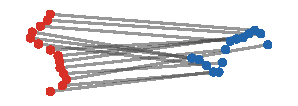
\includegraphics[width=.30\linewidth]{figures/fused-gromov-feature-geometry/feature-ot.pdf} &
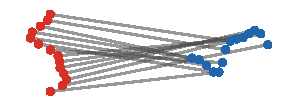
\includegraphics[width=.30\linewidth]{figures/fused-gromov-feature-geometry/fused-gw.pdf} &
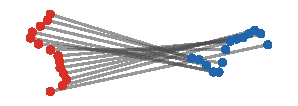
\includegraphics[width=.30\linewidth]{figures/fused-gromov-feature-geometry/pure-gw.pdf}
\end{tabular}
\caption{\emph{Feature information and intrinsic geometry in fused Gromov--Wasserstein.} Small inner disks encode binary node features. Feature-only OT follows the attributes even when this crosses the shape structure, pure GW follows the intrinsic ordering, and fused GW balances the feature term with the pairwise-distance distortion.}
\index{feature term}% strictindex
\index{node feature}% strictindex
\index{distortion}% strictindex
\index{fused Gromov-Wasserstein}% strictindex
\label{fig:fused-gromov-feature-geometry}
\end{figure}

\begin{example}[Application to multi-omics alignment]\label{ex-multi-omics-alignment}
\index{multi-omics}% strictindex
\index{single-cell genomics}% strictindex
	Multi-omics experiments can produce unmatched point clouds in different feature spaces, for instance RNA and ATAC profiles measured on different cells. If direct feature comparison is unavailable or incomplete, the relational term in GW preserves neighborhood structure; if partial cross-feature information exists, fused GW uses it through \(M_{ij}\). Unbalanced and co-optimal variants further allow the number and relative importance of cells or features to differ across modalities. The mathematical template is therefore precise: preserve within-modality geometry while learning a cross-modality coupling~\cite{TranJanatiCourtyFlamaryRedkoDemetciSingh2022UCOOT,RyuBunnePinelloRegevLopez2024LabeledGW,StanojevicLiGarmire2022MultiOmicsReview}.
\end{example}

\Needspace{7\baselineskip}
\paragraph{Hausdorff and Gromov--Hausdorff viewpoints.}
\index{Hausdorff distance}% strictindex
\index{Gromov-Hausdorff distance}% strictindex

Gromov--Hausdorff comparison is the measure-free, worst-case endpoint of intrinsic matching. To make this precise, one must distinguish three feasible objects: arbitrary correspondences for Gromov--Hausdorff, measure-preserving maps for Gromov--Monge, and probability couplings for Gromov--Wasserstein.
\begin{defn}[Hausdorff and Gromov--Hausdorff distances]\label{def-hausdorff-gromov-hausdorff}
If $A,B$ are compact subsets of a metric space $(\Z,\dist_\Z)$, their Hausdorff distance is
\[
	d_{\mathrm H}^{\Z}(A,B)
	=
	\max\left\{
		\sup_{a\in A}\inf_{b\in B}\dist_\Z(a,b),
		\sup_{b\in B}\inf_{a\in A}\dist_\Z(a,b)
	\right\}.
\]
The Gromov--Hausdorff distance removes the common ambient space by minimizing this quantity over all isometric embeddings into a third space:
\index{isometric embedding}% strictindex
\index{Hausdorff distance}% strictindex
\index{Gromov-Hausdorff distance}% strictindex
\[
d_{\mathrm{GH}}(\X,\Y)
=
\inf_{\Z,\phi,\psi}
d_{\mathrm H}^{\Z}(\phi(\X),\psi(\Y)).
\]
A correspondence is a set $R\subset\X\times\Y$ whose two coordinate projections are surjective. Its distortion is
\[
	\operatorname{dis}(R)
	\eqdef
	\sup_{(x,y),(x',y')\in R}
	\abs{\dist_\X(x,x')-\dist_\Y(y,y')}.
\]
For compact metric spaces, the equivalent correspondence formula is
\begin{equation}\label{eq-gh-correspondence-distortion}
	2d_{\mathrm{GH}}(\X,\Y)
	=
	\inf_{R\in\mathfrak R(\X,\Y)}\operatorname{dis}(R),
\end{equation}
where $\mathfrak R(\X,\Y)$ denotes the set of correspondences~\cite{gromov-2001,memoli-2007,memoli-2011}.
\end{defn}

Now equip $\X$ and $\Y$ with full-support probability measures $\alpha$ and $\beta$, and write $\XX=(\X,\dist_\X,\alpha)$ and $\YY=(\Y,\dist_\Y,\beta)$. In this paragraph, $\GW_p$ denotes~\eqref{eq-gw-generic} with $\De(r,s)=|r-s|$. Its Gromov--Monge counterpart restricts the coupling to the graph of a measurable, measure-preserving map:
\begin{equation}\label{eq-gromov-monge-p}
	\GW_p^{\mathrm M}(\XX,\YY)
	\eqdef
	\inf_{T_\sharp\alpha=\beta}
	\left(
		\iint_{\X^2}
		\abs{\dist_\X(x,x')-\dist_\Y(T(x),T(x'))}^p
		\d\alpha(x)\d\alpha(x')
	\right)^{1/p},
\end{equation}
with value $+\infty$ when no such map exists~\cite{MemoliNeedham2024}. Thus Gromov--Monge is directed and may be infinite. For $p=\infty$, the $L^p$ norm is replaced by the essential supremum. Monotonicity of probability-space $L^p$ norms gives, for $1\leq p\leq q<\infty$,
\[
	\GW_p^{\mathrm M}(\XX,\YY)
	\leq
	\GW_q^{\mathrm M}(\XX,\YY)
	\leq
	\GW_\infty^{\mathrm M}(\XX,\YY).
\]
Consequently, $\lim_{p\to\infty}\GW_p^{\mathrm M}$ always exists, but interchanging this limit with the infimum over maps requires additional compactness. The finite case below is one setting where this interchange is immediate. By contrast, weak compactness of the set of couplings makes the Kantorovich limit exact on compact metric-measure spaces.

The Kantorovich counterpart at $p=\infty$ is
\begin{equation}\label{eq-gw-infinity-support}
	\GW_\infty(\XX,\YY)
	\eqdef
	\inf_{\pi\in\Couplings(\alpha,\beta)}
	\operatorname*{ess\,sup}_{\pi\otimes\pi}
	\abs{\dist_\X(x,x')-\dist_\Y(y,y')}
	=
	\inf_{\pi\in\Couplings(\alpha,\beta)}
	\operatorname{dis}(\supp(\pi)).
\end{equation}
The second identity follows from continuity of the distortion integrand. It exposes the exact hierarchy between the three constructions. The factor $2$ below reflects the convention~\eqref{eq-gw-generic}; references that insert a factor $1/2$ in GW do not display it.

\begin{prop}[Gromov--Hausdorff as an infinite-order intrinsic matching]\label{prop-gh-gm-gw-infinity}
	Let $\X$ and $\Y$ be compact metric spaces and let $\alpha,\beta$ have full support. Then
	\begin{equation}\label{eq-gw-p-to-infinity}
		\lim_{p\to\infty}\GW_p(\XX,\YY)
		=
		\GW_\infty(\XX,\YY),
	\end{equation}
	and
	\begin{equation}\label{eq-gh-gw-gm-infinity-chain}
		2d_{\mathrm{GH}}(\X,\Y)
		\leq
		\GW_\infty(\XX,\YY)
		\leq
		\GW_\infty^{\mathrm M}(\XX,\YY).
	\end{equation}
	Moreover, removing the prescribed weights recovers Gromov--Hausdorff exactly:
	\begin{equation}\label{eq-gh-as-weight-envelope-gw-infinity}
		2d_{\mathrm{GH}}(\X,\Y)
		=
		\inf_{\substack{\alpha\in\Mm_+^1(\X),\ \supp(\alpha)=\X\\
		                       \beta\in\Mm_+^1(\Y),\ \supp(\beta)=\Y}}
		\GW_\infty\bigl((\X,\dist_\X,\alpha),(\Y,\dist_\Y,\beta)\bigr).
	\end{equation}
	If $\X=\{x_i\}_{i=1}^n$ and $\Y=\{y_j\}_{j=1}^n$ carry uniform measures, then
	\begin{align}
		\GW_p^{\mathrm M}(\XX,\YY)
		&=
		\min_{\sigma\in\mathfrak S_n}
		\left(
			\frac1{n^2}\sum_{i,i'=1}^n
			\abs{\dist_\X(x_i,x_{i'})-\dist_\Y(y_{\sigma(i)},y_{\sigma(i')})}^p
		\right)^{1/p},
		\label{eq-finite-gromov-monge-p}\\
		\lim_{p\to\infty}\GW_p^{\mathrm M}(\XX,\YY)
		&=
		\GW_\infty^{\mathrm M}(\XX,\YY)
		=
		\GW_\infty(\XX,\YY).
		\label{eq-finite-gw-gm-infinity-limit}
	\end{align}
\end{prop}
\begin{proof}
	The support of any $\pi\in\Couplings(\alpha,\beta)$ is compact. The support of each marginal is the closure of the corresponding coordinate projection of $\supp(\pi)$. These projections are compact, hence already closed; because $\alpha$ and $\beta$ have full support, they are therefore equal to $\X$ and $\Y$. Thus $\supp(\pi)$ is a correspondence, and~\eqref{eq-gh-correspondence-distortion} gives the first inequality in~\eqref{eq-gh-gw-gm-infinity-chain}. Every measure-preserving map generates the graph coupling $(\Id,T)_\sharp\alpha$, which proves the second inequality.

	We next prove~\eqref{eq-gw-p-to-infinity}. The quantities $\GW_p(\XX,\YY)$ are nondecreasing in $p$ and bounded above by $\GW_\infty(\XX,\YY)$, so they converge to some $L\leq\GW_\infty(\XX,\YY)$. Let $p_k\to\infty$. Compactness of $\Couplings(\alpha,\beta)$ and continuity of the bounded distortion integrand ensure the existence of an optimal coupling $\pi_k$ for each finite $p_k$. After extraction, $\pi_k\rightharpoonup\pi_\star$ for some $\pi_\star\in\Couplings(\alpha,\beta)$. Fix $(x,y),(x',y')\in\supp(\pi_\star)$ whose distortion is positive, and choose
	\[
		0<r<\abs{\dist_\X(x,x')-\dist_\Y(y,y')}.
	\]
	By continuity, there are neighborhoods $U$ and $V$ of $(x,y)$ and $(x',y')$ on whose product the distortion exceeds $r$. Since both points belong to $\supp(\pi_\star)$, the Portmanteau theorem gives $\liminf_k\pi_k(U)>0$ and $\liminf_k\pi_k(V)>0$. Hence, for some $c>0$ and all sufficiently large $k$,
	\[
		\GW_{p_k}(\XX,\YY)
		\geq
		r\bigl(\pi_k(U)\pi_k(V)\bigr)^{1/p_k}
		\geq
		rc^{1/p_k}.
	\]
	Letting first $k\to\infty$ and then $r\uparrow\abs{\dist_\X(x,x')-\dist_\Y(y,y')}$ shows that $L$ dominates the distortion of the selected pair. The claim is immediate for pairs of zero distortion. Taking the supremum over $\supp(\pi_\star)^2$ yields
	\[
		L
		\geq
		\operatorname{dis}(\supp(\pi_\star))
		\geq
		\GW_\infty(\XX,\YY),
	\]
	and proves~\eqref{eq-gw-p-to-infinity}.

	For~\eqref{eq-gh-as-weight-envelope-gw-infinity}, the preceding lower bound applies to every pair of full-support weights. Conversely, choose a correspondence $R$ with distortion arbitrarily close to the right-hand side of~\eqref{eq-gh-correspondence-distortion}. Replacing $R$ by its closure preserves both the correspondence property and its distortion, so $R$ may be assumed compact. It then carries a probability $\pi$ with support exactly $R$. Let $\alpha$ and $\beta$ be its marginals. They have full support, while~\eqref{eq-gw-infinity-support} gives $\GW_\infty(\XX,\YY)\leq\operatorname{dis}(R)$. Taking the infimum over $R$ proves the identity.

	For equal-size uniform finite spaces, a measure-preserving map is a permutation, which gives~\eqref{eq-finite-gromov-monge-p}. Since $\mathfrak S_n$ is finite, its minimum commutes with $p\to\infty$. It remains to compare the two infinite-order problems. Let $\P_\infty$ minimize $\GW_\infty$. The scaled matrix $n\P_\infty$ is doubly stochastic, so Theorem~\ref{thm-birkhoff-von-neumann} provides a permutation whose graph is contained in $\supp(\P_\infty)$. Its distortion cannot exceed $\operatorname{dis}(\supp(\P_\infty))=\GW_\infty(\XX,\YY)$. Hence $\GW_\infty^{\mathrm M}\leq\GW_\infty$, while the reverse inequality follows from~\eqref{eq-gh-gw-gm-infinity-chain}. This proves~\eqref{eq-finite-gw-gm-infinity-limit}.
\end{proof}

This makes the relation precise. Gromov--Monge is the hard-map version of GW, and its $p=\infty$ endpoint minimizes the worst distortion induced almost everywhere by a measure-preserving map. In particular, for equal-size uniform finite spaces,
\[
	2d_{\mathrm{GH}}(\X,\Y)
	\leq
	\lim_{p\to\infty}\GW_p^{\mathrm M}(\XX,\YY),
\]
with equality whenever an optimal Gromov--Hausdorff correspondence contains the graph of a bijection. In general, Gromov--Hausdorff allows arbitrary correspondences and ignores prescribed weights, so it can be smaller. Finite-$p$ GW instead averages distortion according to the coupling and can discount low-mass regions; this robustness disappears at $p=\infty$, where every pair in the coupling support contributes to the worst case. The finite-$p$ equality of Gromov--Monge and Gromov--Wasserstein values for nonatomic spaces~\cite{MemoliNeedham2024} does not by itself identify their $p=\infty$ endpoints: approximation of a coupling by graph couplings controls integral distortion, but not necessarily the worst distortion of their supports.
\index{distortion}% strictindex
\index{correspondence}% strictindex
\index{Gromov-Wasserstein@Gromov--Wasserstein}% strictindex
\index{Gromov-Monge@Gromov--Monge}% strictindex
\index{Hausdorff distance}% strictindex

\section{Quantum Optimal Transport}
\index{quantum!OT}% strictindex
\label{sec-quantum-ot}

Quantum optimal transport replaces probability vectors by density matrices and scalar couplings by positive operators on a tensor product space. This is the right language when the transported objects are matrix-valued signals, covariance-like descriptors or quantum states, and it exposes a precise bridge between OT, non-commutative entropy and operator scaling. The finite-dimensional formulation below follows the semidefinite viewpoint developed in matrix-valued and quantum OT~\cite{Ning2014metrics,Chen2016,ChenGangbo17,2016-peyre-qot,caglioti2019quantum,chakrabarti2019quantum}.
\index{positive!operator}% strictindex
\index{quantum!OT}% strictindex
\index{operator scaling}% strictindex
\index{density!matrix}% strictindex

\paragraph{Finite-dimensional states and couplings.}
\index{quantum!coupling}% strictindex

The finite-dimensional case is the cleanest quantum analogue of the Kantorovich formulation. Probability vectors are replaced by positive semidefinite, trace-one matrices, and a coupling becomes a positive semidefinite operator on a tensor product whose partial traces prescribe the two marginals. This keeps the familiar ``joint object with fixed marginals'' geometry, while turning the transport problem into a semidefinite program.

\begin{defn}[Hermitian and density matrices]\label{def-hermitian-density-matrices}
\index{Hermitian matrix}% strictindex
	Let $\mathbb H_n$ be the real vector space of $n\times n$ Hermitian matrices,
	\[
		\mathbb H_n^+
		=
		\enscond{A\in\mathbb H_n}{A\succeq0},
		\qquad
		\mathbb H_n^{+,1}
		=
		\enscond{A\in\mathbb H_n^+}{\tr(A)=1}.
	\]
	Elements of $\mathbb H_n^{+,1}$ are density matrices.
\index{density!matrix}% strictindex
\end{defn}
A joint quantum state between $\CC^n$ and $\CC^m$ is a matrix $T\in\mathbb H_{nm}^+$ acting on $\CC^n\otimes\CC^m$. Its marginals are the partial traces, defined by duality through
\index{trace!partial}% strictindex
\begin{equation}\label{eq-qot-partial-traces}
	\tr(F\,\operatorname{Tr}_B T)=\tr((F\otimes\Id_m)T),
	\qquad
	\tr(G\,\operatorname{Tr}_A T)=\tr((\Id_n\otimes G)T),
\end{equation}
for all $F\in\mathbb H_n$ and $G\in\mathbb H_m$. Thus $\operatorname{Tr}_B(T)\in\mathbb H_n^+$ and $\operatorname{Tr}_A(T)\in\mathbb H_m^+$ play exactly the role of the two marginals of a classical coupling. The feasible set is never empty, since $A\otimes B$ has marginals $A$ and $B$.

\begin{defn}[Finite-dimensional quantum OT]\label{def-finite-dimensional-qot}
\index{quantum!OT}% strictindex
	Let $A\in\mathbb H_n^{+,1}$, $B\in\mathbb H_m^{+,1}$ and let $C\in\mathbb H_{nm}$ be a Hermitian cost observable. The quantum OT value is the semidefinite program
\index{semidefinite program}% strictindex
\index{Hermitian matrix}% strictindex
\index{quantum!OT}% strictindex
	\begin{equation}\label{eq-qot-primal}
		\mathrm{QOT}_C(A,B)
		\eqdef
		\min_{T\in\mathbb H_{nm}^+}
		\enscond{\tr(CT)}{\operatorname{Tr}_B(T)=A,\ \operatorname{Tr}_A(T)=B}.
	\end{equation}
\end{defn}

\begin{example}[Classical diagonal case]\label{rem-qot-classical-diagonal-case}
	Suppose that $A$, $B$ and $C$ are diagonal in fixed product bases. Let $\Delta_A$ and $\Delta_B$ be the corresponding dephasing maps. For every feasible $T$, the matrix $\widetilde T=(\Delta_A\otimes\Delta_B)(T)$ is positive, has the same partial traces, and satisfies $\tr(C\widetilde T)=\tr(CT)$. Hence an optimal coupling may be chosen diagonal. Its diagonal entries form a nonnegative matrix with row sums given by $A$ and column sums given by $B$, so~\eqref{eq-qot-primal} reduces exactly to classical Kantorovich OT. The genuinely quantum feature is that non-commuting data may require off-diagonal coherences or entanglement.
\index{trace!partial constraint}% strictindex
\end{example}


\begin{prop}[Quantum Kantorovich duality]\label{prop-qot-duality}
\index{Kantorovich!duality}% strictindex
\index{quantum!Kantorovich duality}% strictindex
	For $A\in\mathbb H_n^{+,1}$ and $B\in\mathbb H_m^{+,1}$, the dual of~\eqref{eq-qot-primal} is
	\begin{equation}\label{eq-qot-dual}
		\mathrm{QOT}_C(A,B)
		=
		\sup_{F\in\mathbb H_n,\ G\in\mathbb H_m}
		\left\{
			\tr(FA)+\tr(GB)
			:\,
			F\otimes\Id_m+\Id_n\otimes G\preceq C
		\right\}.
	\end{equation}
	There is no duality gap. If $A$ and $B$ are positive definite, the supremum is attained. For singular marginals, the primal reduces to the tensor product of their supports; on this reduced space the corresponding dual maximum is attained, while the full-space formula above is always valid as a supremum.
\index{duality!strong}% strictindex
\index{Slater condition}% strictindex
\end{prop}

\begin{proof}
	Introduce Hermitian Lagrange multipliers $F$ and $G$ for the two marginal constraints. The Lagrangian is
\index{Hermitian matrix}% strictindex
\index{marginal!constraint}% strictindex
	\[
		\tr(CT)+\tr\!\left(F(A-\operatorname{Tr}_B T)\right)
		+\tr\!\left(G(B-\operatorname{Tr}_A T)\right)
		=
		\tr(FA)+\tr(GB)
		+\tr\!\left((C-F\otimes\Id_m-\Id_n\otimes G)T\right),
	\]
	where~\eqref{eq-qot-partial-traces} was used in the last equality. Minimizing over $T\succeq0$ gives a finite lower bound if and only if $C-F\otimes\Id_m-\Id_n\otimes G\succeq0$, in which case the infimum in $T$ is $0$. This gives the dual program. When $A,B\succ0$, the coupling $A\otimes B$ is strictly feasible, so Slater's theorem gives equality of primal and dual values and dual attainment.

	For singular marginals, let $P_A$ and $P_B$ be their support projections. If $T$ is feasible, then
	\[
		\tr\bigl(((\Id_n-P_A)\otimes\Id_m)T\bigr)
		=
		\tr((\Id_n-P_A)A)=0.
	\]
	Positivity implies that $T$ vanishes on $(\supp A)^\perp\otimes\CC^m$; the analogous argument for $B$ yields
	\(T=(P_A\otimes P_B)T(P_A\otimes P_B)\).
	Thus the primal is exactly the problem obtained by compressing $A$, $B$ and $C$ to $\supp A\otimes\supp B$. The reduced marginals are positive definite, so Slater applies there. Equivalently, the unreduced dual values approach the reduced maximum after assigning sufficiently negative potentials on the orthogonal complements. This proves the stated supremum formula without a gap.
\index{Slater condition}% strictindex
\index{dual!attainment}% strictindex
\index{trace!partial}% strictindex
\end{proof}

The dual potentials have the usual scalar gauge freedom: replacing $(F,G)$ by $(F+t\Id_n,G-t\Id_m)$ leaves both the constraint and the value unchanged because $\tr(A)=\tr(B)=1$.
\index{dual!potential}% strictindex

\paragraph{Entropic regularization and Bregman iterations.}
\index{entropic!regularization}% strictindex
\index{Bregman!iteration}% strictindex
As in scalar OT, one obtains a smoother problem by adding the convex quantum entropy functional associated with the matrix logarithm.

\begin{defn}[von Neumann quantum entropy]\label{def-von-neumann-quantum-entropy}
\index{von Neumann entropy}% strictindex
	For a density matrix or positive semidefinite matrix $T$, the shifted von Neumann entropy functional used here is
\index{density!matrix}% strictindex
	\[
		H(T)=\tr\!\left(T(\log T-\Id)\right),
		\qquad
		\nabla H(T)=\log T,
	\]
	with the convention $0\log0=0$ on eigenvalues. This is the convex negative quantum entropy; on trace-one states it differs from the physical entropy $-\tr(T\log T)$ by a sign and an additive constant.
\end{defn}
\eqllead{For $\epsilon>0$ define}{eq-qot-entropic-primal}{
	\mathrm{QOT}_C^\epsilon(A,B)
	=
	\min_{T\succeq0}
	\left\{
		\tr(CT)+\epsilon H(T)
		:\,
		\operatorname{Tr}_B(T)=A,
		\operatorname{Tr}_A(T)=B
	\right\}.
}
This is the non-commutative analogue of entropic OT~\cite{2016-peyre-qot,chakrabarti2019quantum}: the Shannon entropy of a coupling is replaced by the trace entropy of a density matrix.
\index{trace!entropy}% strictindex
\index{entropic!OT}% strictindex
\index{Shannon entropy}% strictindex
\index{density!matrix}% strictindex

\begin{prop}[Entropic quantum OT duality]\label{prop-qot-entropic-duality}
\index{quantum!OT}% strictindex
\index{quantum!OT duality}% strictindex
	Assume $A\succ0$, $B\succ0$ and $\epsilon>0$. Then~\eqref{eq-qot-entropic-primal} has a unique positive minimizer. Its dual is
	\begin{equation}\label{eq-qot-entropic-dual}
		\mathrm{QOT}_C^\epsilon(A,B)
		=
		\max_{F\in\mathbb H_n,\ G\in\mathbb H_m}
		\left\{
			\tr(FA)+\tr(GB)
			-\epsilon\,
			\tr\exp\!\left(\frac{F\otimes\Id_m+\Id_n\otimes G-C}{\epsilon}\right)
		\right\}.
	\end{equation}
	At optimality, primal and dual variables are linked by the Gibbs formula
\index{Gibbs!formula}% strictindex
	\begin{equation}\label{eq-qot-gibbs-coupling}
		T_e(F,G)
		=
		\exp\!\left(\frac{F\otimes\Id_m+\Id_n\otimes G-C}{\epsilon}\right),
	\end{equation}
	with $\operatorname{Tr}_B(T_e)=A$ and $\operatorname{Tr}_A(T_e)=B$.
\end{prop}

\begin{proof}
	The feasible set is compact and nonempty, and it contains the positive definite point $A\otimes B$. The trace entropy is strictly convex on positive semidefinite matrices, hence the regularized primal has a unique minimizer. This minimizer is positive definite: if it had a non-trivial kernel, moving toward $A\otimes B$ would have entropy directional derivative $-\infty$ at the boundary while changing the linear cost only at finite rate. Slater's condition justifies the Lagrange dual computation. The Fenchel identity
\index{trace!entropy}% strictindex
\index{Slater condition}% strictindex
\index{positive!semidefinite matrix}% strictindex
	\[
		\sup_{T\succeq0}\ \tr(YT)-\epsilon H(T)
		=
		\epsilon\,\tr\exp(Y/\epsilon)
	\]
	is the matrix analogue of the scalar exponential conjugacy. Applying it to the Lagrangian of~\eqref{eq-qot-entropic-primal}, with
	$Y=F\otimes\Id_m+\Id_n\otimes G-C$, gives~\eqref{eq-qot-entropic-dual}. The stationarity condition of this Fenchel identity gives~\eqref{eq-qot-gibbs-coupling}; differentiating the dual objective with respect to $F$ and $G$ yields the two marginal equations.
\index{stationarity}% strictindex
\index{Gibbs!coupling}% strictindex
\end{proof}

Writing $K=\exp(-C/\epsilon)$, the objective in~\eqref{eq-qot-entropic-primal} differs by a constant from $\epsilon$ times the quantum KL divergence
\[
	D_H(T|K)
	=
	\tr\!\left(T(\log T-\log K)-T+K\right).
\]
The exact quantum analogue of Sinkhorn is an implicit alternating Bregman projection scheme onto the affine marginal sets
\index{Bregman!projection}% strictindex
\[
	\mathcal M_A=\{T\succeq0:\operatorname{Tr}_B(T)=A\},
	\qquad
	\mathcal M_B=\{T\succeq0:\operatorname{Tr}_A(T)=B\}.
\]

\begin{prop}[Exact Bregman projections]\label{prop-qot-bregman-projections}
	Assume $A,B\succ0$ and let $K=\exp(-C/\epsilon)$. The minimizer of~\eqref{eq-qot-entropic-primal} is equivalently the minimizer of $D_H(T|K)$ over $\mathcal M_A\cap\mathcal M_B$. Moreover, if a current positive definite matrix has Gibbs form $T_e(F,G)$, then its Bregman projection onto $\mathcal M_A$ has the form $T_e(F^+,G)$, where $F^+$ is chosen so that $\operatorname{Tr}_B T_e(F^+,G)=A$. The projection onto $\mathcal M_B$ is analogous. Thus, when each one-block marginal equation is solved exactly, alternating Bregman projections are equivalent to alternating block maximization of the dual~\eqref{eq-qot-entropic-dual}.
\end{prop}

\begin{proof}
	Since $\log K=-C/\epsilon$, the identity
	\[
		\tr(CT)+\epsilon H(T)
		=
		\epsilon D_H(T|K)-\epsilon\tr(K)
	\]
	holds, so the primal minimizer is the constrained Bregman projection of $K$ up to an additive constant. For the projection of a positive definite matrix $S$ onto $\mathcal M_A$, the affine set contains the positive definite point $A\otimes\Id_m/m$; the entropy derivative $\log T-\log S$ is singular at the boundary, so the projection lies in the interior of the positive cone. Its Lagrangian first variation is
\index{first variation}% strictindex
\index{Bregman!projection}% strictindex
\index{positive!cone}% strictindex
	\(\log T-\log S-\Lambda\otimes\Id_m=0\)
	for a Hermitian multiplier $\Lambda$. Hence $T=\exp(\log S+\Lambda\otimes\Id_m)$. If $S=T_e(F,G)$, this is again of the form $T_e(F+\epsilon\Lambda,G)$. The multiplier is fixed by the marginal equation $\operatorname{Tr}_B(T)=A$. The same argument applies to $\mathcal M_B$. Finally, the first-order optimality condition for maximizing~\eqref{eq-qot-entropic-dual} over one block is exactly the corresponding marginal equation, so the Bregman and block-dual views coincide.
\index{Hermitian matrix}% strictindex
\index{optimality!first-order}% strictindex
\end{proof}

In the diagonal case this proposition gives the usual multiplicative Sinkhorn updates. In the non-commutative case, however, the exact block equations
\index{Sinkhorn!update}% strictindex
\[
	\operatorname{Tr}_B T_e(F,G)=A,
	\qquad
	\operatorname{Tr}_A T_e(F,G)=B
\]
do not admit scalar division formulas, because the exponential of $F\otimes\Id_m+\Id_n\otimes G-C$ cannot be separated unless the local potential $F\otimes\Id_m+\Id_n\otimes G$ commutes with the cost $C$.
When all matrices are diagonal in the same basis, commutativity restores the scalar form $T_e=\diag(u)K\diag(v)$ and the marginal equations reduce to the usual Sinkhorn divisions.

Algorithm~\ref{alg:quantum-exact-bregman} records this exact but implicit non-commutative analogue of Sinkhorn.

\begin{alg}[Exact quantum Bregman projections]\label{alg:quantum-exact-bregman}
\index{Bregman!projection}% strictindex
\index{quantum!Bregman projection}% strictindex
\textbf{Input:} Positive definite density matrices $A,B$, cost $C$, regularization $\epsilon>0$, tolerance $\mathrm{tol}$, iteration budget $L\geq1$.

\textbf{Output:} Approximate quantum entropic coupling $T$ and its partial-trace residual.

\textbf{Initialize:} Set Hermitian potentials $F^{(0)}=0$ and $G^{(0)}=0$.

\textbf{For} $\ell=0,\ldots,L-1$ \textbf{do}:
\begin{algblock}
\(T^{(\ell)}= T_e(F^{(\ell)},G^{(\ell)}) = \exp\!\left( \frac{F^{(\ell)}\otimes\Id_m+\Id_n\otimes G^{(\ell)}-C}{\epsilon} \right)\).

\textbf{Solve} $A$-projection equation:
\(\operatorname{Tr}_B T_e(F^+,G^{(\ell)})=A\).

\textbf{Set} $F^{(\ell+1)}=F^+$.

\textbf{Solve} $B$-projection equation:
\(\operatorname{Tr}_A T_e(F^{(\ell+1)},G^+)=B\).

\textbf{Set} $G^{(\ell+1)}=G^+$.

\textbf{Set} $T^{(\ell+1)}=T_e(F^{(\ell+1)},G^{(\ell+1)})$ and
\(r^{(\ell+1)}=\max\{\norm{\operatorname{Tr}_B T^{(\ell+1)}-A}_{\mathrm F},\norm{\operatorname{Tr}_A T^{(\ell+1)}-B}_{\mathrm F}\}.\)

\textbf{If} $r^{(\ell+1)}\leq\mathrm{tol}$ \textbf{then}:
\begin{algblock}
\textbf{Return} $T^{(\ell+1)}$ and $r^{(\ell+1)}$.
\end{algblock}
\end{algblock}
\algreturnskip
\textbf{Return} $T^{(L)}$ and $r^{(L)}$.
\end{alg}

\paragraph{Gurvits scaling and quantum Sinkhorn.}
\index{Gurvits scaling}% strictindex
\index{quantum!Sinkhorn}% strictindex
The algorithm often called quantum Sinkhorn comes from the operator-scaling literature of Gurvits and subsequent developments~\cite{gurvits2003classical,gurvits2004classical,georgiou2015positive,garg2018recent}. It replaces the true Gibbs coupling~\eqref{eq-qot-gibbs-coupling} by the symmetric factorization
\index{operator scaling}% strictindex
\index{Gibbs!coupling}% strictindex
\begin{equation}\label{eq-qot-symmetric-scaling}
	T_s(F,G)
	=
	\exp\!\left(\frac{Z}{2\epsilon}\right)\exp(-C/\epsilon)\exp\!\left(\frac{Z}{2\epsilon}\right)
	=
	(U\otimes V)K(U\otimes V),
	\qquad
	Z=F\otimes\Id_m+\Id_n\otimes G,
\end{equation}
where $U=\exp(F/(2\epsilon))$, $V=\exp(G/(2\epsilon))$ and $K=\exp(-C/\epsilon)$. If $[Z,C]=0$, then $T_s(F,G)=T_e(F,G)$; otherwise this is a Strang-type symmetric surrogate.
\index{Strang splitting}% strictindex

Fix a Choi convention and let $\mathcal K:\mathbb H_m\to\mathbb H_n$ be the completely positive map represented by the positive Choi matrix $K$; let $\mathcal K^\star$ be its Hilbert--Schmidt adjoint. Up to the transpose dictated by the chosen Choi convention, the marginal equations for the symmetric coupling take the operator-scaling form
\index{Choi matrix}% strictindex
\index{operator scaling}% strictindex
\index{scaling!form}% strictindex
\[
	U\,\mathcal K(V^2)\,U=A,
	\qquad
	V\,\mathcal K^\star(U^2)\,V=B.
\]
They can be enforced by the explicit congruence normalizations
\index{congruence normalization}% strictindex
\begin{equation}\label{eq-qot-gurvits-updates}
\begin{aligned}
	R_V&=\mathcal K(V^2),
	&
	U&\leftarrow
	R_V^{-1/2}\bigl(R_V^{1/2} A R_V^{1/2}\bigr)^{1/2}R_V^{-1/2},
	\\
	S_U&=\mathcal K^\star(U^2),
	&
	V&\leftarrow
	S_U^{-1/2}\bigl(S_U^{1/2} B S_U^{1/2}\bigr)^{1/2}S_U^{-1/2}.
\end{aligned}
\end{equation}
\begin{alg}[Gurvits/operator scaling for quantum Sinkhorn]\label{alg:quantum-gurvits-scaling}
\index{operator scaling}% strictindex
\textbf{Input:} Positive definite marginals $A,B$, positive definite kernel operator $K$, maps $\mathcal K,\mathcal K^\star$, tolerance $\mathrm{tol}$, iteration budget $L\geq1$.

\textbf{Output:} Symmetrically scaled coupling $T_s$ and its marginal residual $r$.

\textbf{Initialize:} Set $U=\Id_n$ and $V=\Id_m$.

\textbf{Set} residual \(r=+\infty\) and counter $\ell=0$.

\textbf{While} \(r>\mathrm{tol}\) and $\ell<L$ \textbf{do}:
\begin{algblock}
\(R_V=\mathcal K(V^2), \qquad U\leftarrow R_V^{-1/2}\bigl(R_V^{1/2} A R_V^{1/2}\bigr)^{1/2}R_V^{-1/2}\).

\(S_U=\mathcal K^\star(U^2), \qquad V\leftarrow S_U^{-1/2}\bigl(S_U^{1/2} B S_U^{1/2}\bigr)^{1/2}S_U^{-1/2}\).

\textbf{Set} \(T_s=(U\otimes V)K(U\otimes V)\) and \(r\) to the maximum of its two operator-marginal residuals against $A$ and $B$.

\textbf{Set} $\ell\leftarrow \ell+1$.
\end{algblock}
\algreturnskip
\textbf{Return} \(T_s\) and $r$.
\end{alg}
These inverse square roots are well-defined when $K\succ0$ and $U,V,A,B\succ0$. Under the standard strict-positivity and scalability hypotheses, the alternating normalizations converge to the prescribed marginals~\cite{georgiou2015positive,garg2018recent}; the finite algorithm returns once the residual is below tolerance or the iteration budget is exhausted. This is Gurvits/operator scaling with prescribed targets. When all matrices are diagonal it reduces to classical Sinkhorn scaling, and when the targets are proportional to identities it matches the usual bistochastic operator-scaling normalization, up to the conventional trace normalization.
\index{Gurvits scaling}% strictindex
\index{inverse square root}% strictindex
\index{Sinkhorn!scaling}% strictindex
\index{operator scaling}% strictindex


\begin{rem}[Gurvits scaling is not the exact Bregman scheme]
	It is important not to identify~\eqref{eq-qot-gurvits-updates} with the exact Bregman scheme for~\eqref{eq-qot-entropic-primal}. The exact Bregman step would enforce the marginals of $T_e(F,G)=\exp((Z-C)/\epsilon)$ and would be a block maximization of the true concave dual~\eqref{eq-qot-entropic-dual}. Gurvits scaling instead enforces the marginals of the surrogate
\[
	T_s=
	\exp\!\left(\frac{Z}{2\epsilon}\right)
	\exp(-C/\epsilon)
	\exp\!\left(\frac{Z}{2\epsilon}\right).
\]
	The two coincide in the commuting/diagonal regime, but in general the Baker--Campbell--Hausdorff commutator terms do not vanish. The Gurvits iteration should therefore be understood as a tractable symmetric operator-scaling approximation to entropic Q--OT, not as the literal alternating KL projection algorithm.
\index{Gurvits scaling}% strictindex
\index{commutator}% strictindex
\index{Baker-Campbell-Hausdorff formula}% strictindex
\index{operator scaling}% strictindex
\index{KL!projection}% strictindex
\end{rem}

\begin{rem}[Operator-valued couplings]
\index{operator-valued coupling}% strictindex
	The same definitions extend formally from matrices to separable Hilbert spaces by replacing density matrices with positive trace-class operators of trace one, observables with bounded self-adjoint operators and~\eqref{eq-qot-partial-traces} with partial traces defined by duality against local bounded observables. If $\Pi(A,B)$ denotes positive trace-class operators with partial traces $A$ and $B$, a bounded cost observable $C$ gives the problem $\inf_{T\in\Pi(A,B)}\Tr(CT)$. For unbounded positive costs one must define the energy through the quadratic form or spectral truncations, and in the entropic case one must ensure that the Gibbs operator $\exp(-C/\epsilon)$ is trace class and that the partial traces of the candidate coupling are well-defined. The matrix formulas above are therefore the clean finite-dimensional core; the operator version adds domain and compactness assumptions rather than a different algebraic structure.
\index{density!matrix}% strictindex
\index{trace-class operator}% strictindex
\index{trace!partial}% strictindex
\end{rem}

%%%%%%%%%%%%%%%%%%%%%%%%%%%%%%%%%%%%%%%%%%%%%%%%%%%%%%%%%%%%%%%%%%%%%%%%%%%
\section{Dynamic Time Warping}\label{sec-dynamic-time-warping}
\index{dynamic time warping}% strictindex
\index{time series!alignment}% strictindex

Dynamic time warping (DTW) compares ordered feature sequences when the same phenomenon may be observed under different clocks. It is historically rooted in speech recognition~\cite{Vintsyuk1968DTW,SakoeChiba1978DTW}, and is now a standard tool for time-series alignment, retrieval and classification~\cite{BerndtClifford1994DTW,Muller2007MusicMotion}. Like OT, it minimizes an aggregate feature mismatch over correspondences; unlike OT, those correspondences must respect chronology.

\paragraph{Ordered alignments versus transport couplings.}
For two empirical measures, Kantorovich OT minimizes a linear cost over the convex polytope of nonnegative matrices with prescribed row and column sums. DTW instead minimizes over the finite, non-convex set of connected monotone paths through the pairwise cost matrix. Every time index must be visited, but it may be visited repeatedly; the row and column sums therefore record endogenous visit counts rather than prescribed masses. Normalizing a path matrix produces a coupling only for these path-dependent marginals, not for fixed input histograms. Conversely, ordinary OT between the unordered empirical feature measures forgets chronology and may match indices in a crossing order. Temporal penalties, causal constraints, and joint OT--DTW models interpolate between the two viewpoints; for example, spatio-temporal alignment combines regularized OT for spatial comparison with soft-DTW for chronological alignment~\cite{JanatiCuturiGramfort2020STA}. Here ``dynamic'' refers to Bellman's dynamic programming on the index grid, not to the transport PDEs of Chapter~\ref{sec-dynamic-optimal-transport}.
\index{transport!coupling}% strictindex
\index{monotone!alignment}% strictindex

\paragraph{Discrete variational problem.}
Let $x=(x_i)_{i=1}^n$ and $y=(y_j)_{j=1}^m$ be two sequences in a feature space $\mathcal Z$, and set $\C_{ij}=c(x_i,y_j)$ for a nonnegative cost $c:\mathcal Z\times\mathcal Z\to\RR_+$. A warping path is a sequence
\[
	\omega=((i_\ell,j_\ell))_{\ell=1}^L
\]
that starts at $(1,1)$, ends at $(n,m)$, and has increments
\[
	(i_{\ell+1}-i_\ell,j_{\ell+1}-j_\ell)
	\in\{(1,0),(0,1),(1,1)\}.
\]
Denote the set of such paths by $\Omega_{n,m}$ and the corresponding incidence matrix by $(A_\omega)_{ij}=\mathbf 1_{\{(i,j)\in\omega\}}$. Its length satisfies $\max\{n,m\}\leq L\leq n+m-1$, its total mass is $\sum_{ij}(A_\omega)_{ij}=L$, and its two marginals are precisely the row and column visit counts.

\begin{defn}[Dynamic time warping]\label{def-dynamic-time-warping}
\index{warping path}% strictindex
	The DTW value associated with the feature cost $c$ is
	\begin{equation}\label{eq-dtw-variational}
		\mathrm{DTW}_c(x,y)
		\eqdef
		\min_{\omega\in\Omega_{n,m}}
		\sum_{\ell=1}^L c(x_{i_\ell},y_{j_\ell})
		=
		\min_{\omega\in\Omega_{n,m}}\dotp{A_\omega}{\C}.
	\end{equation}
\end{defn}
The definition is symmetric when $c$ is symmetric, but it is generally not a metric: repetitions can give zero cost to distinct sequences, and the triangle inequality can fail. Step weights, slope constraints and a Sakoe--Chiba band are common variants that penalize excessive repetition or restrict the admissible temporal distortion~\cite{SakoeChiba1978DTW,Muller2007MusicMotion}.
\index{Sakoe--Chiba band}% strictindex

\paragraph{Dynamic programming.}
The monotone path structure converts the exponentially large variational problem~\eqref{eq-dtw-variational} into a shortest-path computation on an acyclic grid.

\begin{prop}[DTW dynamic-programming recurrence]\label{prop-dtw-dynamic-programming}
\index{dynamic programming}% strictindex
	Set $D_{0,0}=0$, $D_{i,0}=D_{0,j}=+\infty$ for $i,j>0$, and, for $1\leq i\leq n$, $1\leq j\leq m$, define
	\begin{equation}\label{eq-dtw-recurrence}
		D_{ij}
		=
		\C_{ij}+\min\{D_{i-1,j},D_{i,j-1},D_{i-1,j-1}\}.
	\end{equation}
	Then $D_{nm}=\mathrm{DTW}_c(x,y)$. Storing one minimizing predecessor at every cell and backtracking from $(n,m)$ recovers an optimal path. The computation takes $O(nm)$ time and $O(nm)$ memory; if only the value is required, two rows give $O(\min\{n,m\})$ memory.
\end{prop}

\begin{proof}
	Every admissible path reaching $(i,j)$ enters it from exactly one of $(i-1,j)$, $(i,j-1)$ or $(i-1,j-1)$. Removing the last cell therefore leaves an admissible path to one of these predecessors, while appending $(i,j)$ to any predecessor path gives an admissible path to $(i,j)$. Minimizing over the three mutually exhaustive last steps proves~\eqref{eq-dtw-recurrence} by induction on $i+j$. The complexity follows because each of the $nm$ cells performs constant work.
\end{proof}

Algorithm~\ref{alg-dtw-dynamic-programming} makes the value computation and path recovery explicit.

\begin{alg}[Dynamic time warping by dynamic programming]\label{alg-dtw-dynamic-programming}
\index{dynamic time warping!algorithm}% strictindex
\textbf{Input:} Sequences $x=(x_i)_{i=1}^n$, $y=(y_j)_{j=1}^m$, local cost $c$.

\textbf{Output:} DTW value $D_{nm}$ and an optimal warping path $\omega^\star$.

\textbf{Initialize:} Set $D\in(\RR\cup\{+\infty\})^{(n+1)\times(m+1)}$ to $+\infty$, $D_{0,0}=0$, and allocate predecessors $B$.

\textbf{For} $i=1,\ldots,n$ \textbf{do}:
\begin{algblock}
\textbf{For} $j=1,\ldots,m$ \textbf{do}:
\begin{algblock}
\textbf{Set} $\C_{ij}=c(x_i,y_j)$.

\textbf{Choose} the lexicographically first
$(r^\star,s^\star)\in\argmin_{(r,s)\in\{(i-1,j),(i,j-1),(i-1,j-1)\}}D_{rs}$.

\textbf{Set} $B_{ij}=(r^\star,s^\star)$ and $D_{ij}=\C_{ij}+D_{r^\star,s^\star}$.
\end{algblock}
\end{algblock}
\textbf{Initialize:} Set $(i,j)=(n,m)$ and $\omega^\star=[\,]$.

\textbf{While} $(i,j)\neq(0,0)$ \textbf{do}:
\begin{algblock}
\textbf{Prepend} $(i,j)$ to $\omega^\star$.

\textbf{Set} $(i,j)\leftarrow B_{ij}$.
\end{algblock}
\algreturnskip
\textbf{Return} $D_{nm}$ and $\omega^\star$.
\end{alg}

\paragraph{Continuous time warping.}
Discrete DTW depends on the sampling density because every visited cell contributes once. A direct continuous registration minimizes $\int_0^1 c(x(t),y(\gamma(t)))\d t$ over nondecreasing endpoint-fixing maps $\gamma$, but this one-clock formulation is asymmetric and privileges the parameterization of $x$. Continuous DTW instead traverses both clocks and measures mismatch per unit length in the parameter square~\cite{BuchinNusserWong2022CDTW}.

For simplicity, let $x,y:[0,1]\to\mathcal Z$ use normalized clocks. The symmetric continuous registration problem uses two monotone clocks.
\begin{defn}[Continuous dynamic time warping]\label{def-continuous-dtw}
Let $\Gamma_\uparrow$ contain pairs $(\phi,\psi)$ of absolutely continuous, nondecreasing surjections of $[0,1]$ onto itself. Define
\begin{equation}\label{eq-continuous-dtw}
	\mathrm{CDTW}_c(x,y)
	\eqdef
	\inf_{(\phi,\psi)\in\Gamma_\uparrow}
	\int_0^1
	c\bigl(x(\phi(s)),y(\psi(s))\bigr)
	\bigl(\dot\phi(s)+\dot\psi(s)\bigr)\d s.
\end{equation}
\end{defn}
\index{continuous DTW}% strictindex
The surjections satisfy $\phi(0)=\psi(0)=0$ and $\phi(1)=\psi(1)=1$. Because $\dot\phi,\dot\psi\geq0$ almost everywhere, the last factor is the $\ell^1$ line element of the monotone path $s\mapsto(\phi(s),\psi(s))$. Formula~\eqref{eq-continuous-dtw} is invariant under increasing reparameterizations of the auxiliary variable $s$ and does not privilege either clock; when $c$ is symmetric, the resulting functional is also symmetric in $x$ and $y$. After parameterization by $\ell^1$ arc length, it is simply the line integral of the feature mismatch along a monotone path. For physical clock intervals $[0,p]$ and $[0,q]$, the same formula uses $\phi:[0,1]\to[0,p]$ and $\psi:[0,1]\to[0,q]$. Exact computation is substantially harder than the discrete recurrence: for arc-length-parametrized one-dimensional polygonal curves and the standard cost $c(u,v)=\abs{u-v}$, Buchin, Nusser and Wong propagate piecewise-quadratic boundary costs in $O((n+m)^5)$ time~\cite{BuchinNusserWong2022CDTW}. This complexity statement does not apply to an arbitrary feature cost $c$.

\paragraph{Soft-DTW and the Sinkhorn analogy.}
The hard minimum in~\eqref{eq-dtw-recurrence} is nonsmooth when several paths tie. Soft-DTW replaces it with the log-sum-exp soft minimum~\cite{CuturiBlondel2017SoftDTW},
\begin{equation}\label{eq-dtw-softmin}
	\operatorname{softmin}_\epsilon(r_1,\ldots,r_q)
	=
	-\epsilon\log\!\left(\sum_{k=1}^q e^{-r_k/\epsilon}\right),
\end{equation}
and defines $D_{00}^\epsilon=0$, $D_{i0}^\epsilon=D_{0j}^\epsilon=+\infty$ for $i,j>0$, together with
\begin{equation}\label{eq-soft-dtw-recurrence}
	D_{ij}^\epsilon
	=
	\C_{ij}
	+
	\operatorname{softmin}_\epsilon
	\bigl(D_{i-1,j}^\epsilon,D_{i,j-1}^\epsilon,D_{i-1,j-1}^\epsilon\bigr),
	\qquad
	\mathrm{sDTW}_{c,\epsilon}(x,y)=D_{nm}^\epsilon.
\end{equation}
\index{soft-DTW}% strictindex
Equivalently, it is the free energy of all monotone paths,
\begin{equation}\label{eq-soft-dtw-partition}
	\mathrm{sDTW}_{c,\epsilon}(x,y)
	=
	-\epsilon\log
	\sum_{\omega\in\Omega_{n,m}}
	\exp\!\left(-\frac{\dotp{A_\omega}{\C}}{\epsilon}\right).
\end{equation}
To make the regularization explicit, let $\Delta(\Omega_{n,m})$ be the simplex of probability laws $q=(q_\omega)_\omega$ over paths and let $H(q)=-\sum_\omega q_\omega\log q_\omega$ be their Shannon entropy, with $0\log0=0$. The Gibbs variational identity gives
\begin{equation}\label{eq-soft-dtw-variational}
	\mathrm{sDTW}_{c,\epsilon}(x,y)
	=
	\min_{q\in\Delta(\Omega_{n,m})}
	\left\{
	\sum_{\omega}q_\omega\dotp{A_\omega}{\C}
	-\epsilon H(q)
	\right\}.
\end{equation}
\index{path entropy}% strictindex
Its unique minimizer is the Gibbs law
\index{Gibbs!path law}% strictindex
\begin{equation}\label{eq-soft-dtw-gibbs-law}
	\PP_\epsilon(\omega)
	=
	\frac{\exp(-\dotp{A_\omega}{\C}/\epsilon)}
	{\sum_{\omega'}\exp(-\dotp{A_{\omega'}}{\C}/\epsilon)},
	\qquad
	E_\epsilon
	\eqdef
	\nabla_\C\mathrm{sDTW}_{c,\epsilon}(x,y).
\end{equation}
Indeed, subtracting the value in~\eqref{eq-soft-dtw-partition} from the objective in~\eqref{eq-soft-dtw-variational} gives $\epsilon\KL(q|\PP_\epsilon)\geq0$. Moreover,
\begin{equation}\label{eq-soft-dtw-zero-temperature-bound}
	\mathrm{DTW}_c(x,y)-\epsilon\log\abs{\Omega_{n,m}}
	\leq
	\mathrm{sDTW}_{c,\epsilon}(x,y)
	\leq
	\mathrm{DTW}_c(x,y),
\end{equation}
because the partition sum is bounded below by its largest term and above by $\abs{\Omega_{n,m}}$ times that term. Hence $\mathrm{sDTW}_{c,\epsilon}\to\mathrm{DTW}_c$ as $\epsilon\to0$. Forward and backward dynamic programs compute its value and gradient in $O(nm)$ time and $O(nm)$ memory~\cite{CuturiBlondel2017SoftDTW}. Differentiating the finite log-partition function gives
\begin{equation}\label{eq-soft-dtw-expected-alignment}
	E_\epsilon
	=
	\EE_{\omega\sim\PP_\epsilon}[A_\omega].
\end{equation}
Thus $(E_\epsilon)_{ij}$ is the probability that a Gibbs path visits cell $(i,j)$. The matrix $E_\epsilon$ is a diffuse expected alignment and converges, when the hard optimum is unique, to its path-incidence matrix.

The analogy with entropic OT is now exact at the level of free energies, but not at the level of feasible variables. Sinkhorn regularizes a coupling with prescribed marginals, whereas soft-DTW regularizes the path law $q$ in~\eqref{eq-soft-dtw-variational}. Its mean $E_\epsilon$ generally has neither prescribed row sums nor prescribed column sums, and the path entropy $H(q)$ cannot in general be recovered from $E_\epsilon$ alone. Algorithmically, Sinkhorn uses alternating matrix scaling, while soft-DTW uses forward--backward dynamic programming on an acyclic grid. Global-alignment kernels sum the same Gibbs weights over all paths~\cite{CuturiVertBirkenesMatsui2007GlobalAlignment,Cuturi2011GlobalAlignment}.

Raw soft-DTW also has an entropic self-bias and can be negative. In direct analogy with the Sinkhorn divergence of Section~\ref{sec-sinkhorn-div}, the soft-DTW divergence is
\begin{equation}\label{eq-soft-dtw-divergence}
	\overline{\mathrm{sDTW}}_{c,\epsilon}(x,y)
	=
	\mathrm{sDTW}_{c,\epsilon}(x,y)
	-\frac12\mathrm{sDTW}_{c,\epsilon}(x,x)
	-\frac12\mathrm{sDTW}_{c,\epsilon}(y,y).
\end{equation}
The correction always vanishes on the diagonal, but positivity requires care.

\begin{rem}[Validity of the soft-DTW divergence]\label{rem-soft-dtw-divergence-validity}
	Blondel, Mensch and Vert prove that~\eqref{eq-soft-dtw-divergence} is nonnegative and vanishes only for identical sequences when either $c(u,v)=\abs{u-v}$ in one dimension or
	\[
		c(u,v)=\delta(u,v)+\log\!\bigl(2-e^{-\delta(u,v)}\bigr),
		\qquad
		\delta(u,v)=\tfrac12\norm{u-v}^2.
	\]
	For the ordinary squared Euclidean cost used in Figure~\ref{fig:dynamic-time-warping}, they prove for equal-length sequences that the diagonal is stationary and provide numerical evidence for nonnegativity, but do not prove it in general~\cite{BlondelMenschVert2021SoftDTW}. Thus debiasing alone should not be taken as a universal positivity theorem. Even for the costs covered by the result, no triangle inequality is asserted.
\end{rem}

Figure~\ref{fig:dynamic-time-warping} contrasts the hard minimizing path with the expected alignment~\eqref{eq-soft-dtw-expected-alignment} on an exactly time-warped oscillatory signal.

\begin{figure}[ht]
\centering
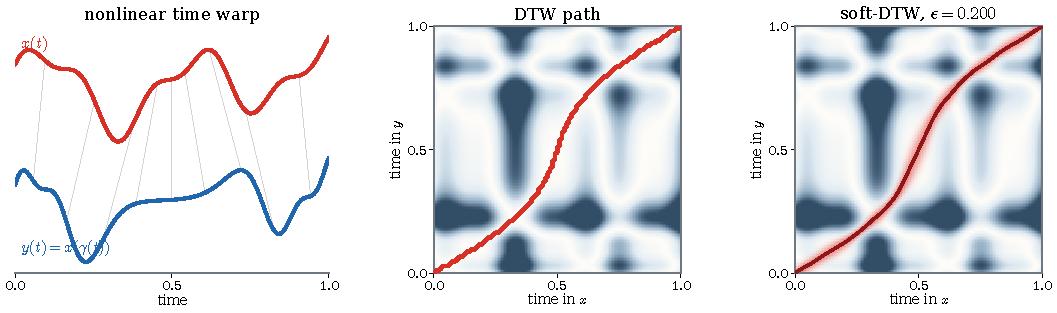
\includegraphics[width=.98\linewidth]{figures/dynamic-time-warping/dtw-alignment.pdf}
\caption{\emph{Hard and soft monotone alignments recover a nonlinear time warp.} Left: an oscillatory signal $x$ and the warped observation $y(t)=x(\gamma(t))$ for a smooth increasing map $\gamma$; thin gray segments mark exact corresponding times. Middle: the pairwise squared feature-cost matrix $\C_{ij}=\abs{x_i-y_j}^2$, with the optimal DTW path shown in red. Right: the same matrix overlaid with the soft-DTW expected alignment $E_\epsilon$ from~\eqref{eq-soft-dtw-expected-alignment} at $\epsilon=.200$; red intensity gives cell-visit probability and the dark red curve is its row-wise barycentric summary.}
\label{fig:dynamic-time-warping}
\index{dynamic time warping!numerics}% strictindex
\index{soft-DTW!expected alignment}% strictindex
\end{figure}
